\section{Die Gauss'sche Zahlenebene}
\subsection{Zahlen in der Zahlenebene}
Während Ihrer gesamten Schulzeit hat Sie die Zahlengerade als geometrisches Modell für Zahlen begleitet. Hierdurch kann man sich Zahlen als Punkte auf der Zahlengeraden vorstellen. 

\textit{Zahlengerade:} Auf der Zahlengeraden finden Sie Punkte für $2$, für $-4$, für $\frac{1}{3}$, für $\sqrt{2}$, für $\pi$ etc. 

\begin{center}
    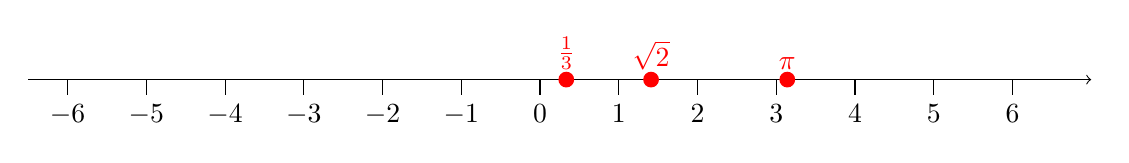
\begin{tikzpicture}
        % Zeichne die Zahlengerade
        \draw[->] (-6.5,0) -- (7,0) node[below] {};
        
        % Markierungen für ganze Zahlen
        \foreach \x in {-6,-5,-4,-3,-2,-1,0,1,2,3,4,5,6}
            \draw (\x,0) -- (\x,-0.2) node[below] {$\x$};
        
        % Markierungen für spezielle Zahlen
        \fill[red] (1/3,0) circle (0.1) node[above] {$\frac{1}{3}$};
        \fill[red] (1.41, 0) circle (0.1) node[above] {$\sqrt{2}$};
        \fill[red] (3.14, 0) circle (0.1) node[above] {$\pi$};


    \end{tikzpicture}
\end{center}



% \begin{center}
%     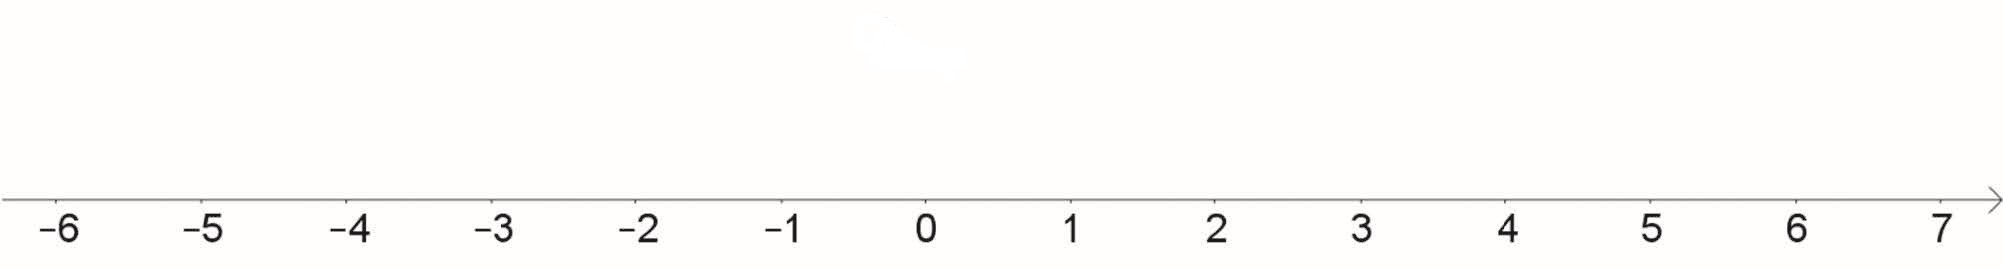
\includegraphics[width = 0.9 \textwidth]{media/Zahlengeradeo.jpg}
% \end{center}

Die imaginäre Einheit $i$ hat aber auf der Zahlengeraden keinen Platz!

Es war eine geniale und bahnbrechende Idee des Mathematikers Carl Friedrich Gauss (1777 – 1855), die Zahlengerade ins Zweidimensionale zu erweitern und der Zahl $i$ in der Ebene einen Platz oberhalb der Null zu geben:

\begin{center}
    \begin{tikzpicture}
        % Zeichne die Zahlengerade
        \draw[->] (-6.5,0) -- (7,0) node[below] {};
        
        % Markierungen für ganze Zahlen
        \foreach \x in {-6,-5,-4,-3,-2,-1,0,1,2,3,4,5,6}
            \draw (\x,0) -- (\x,-0.2) node[below] {$\x$};
        
        % Markierungen für spezielle Zahlen
        \fill[red] (0,1) circle (0.1) node[above] {$i$};



    \end{tikzpicture}
\end{center}
% \begin{center}
%     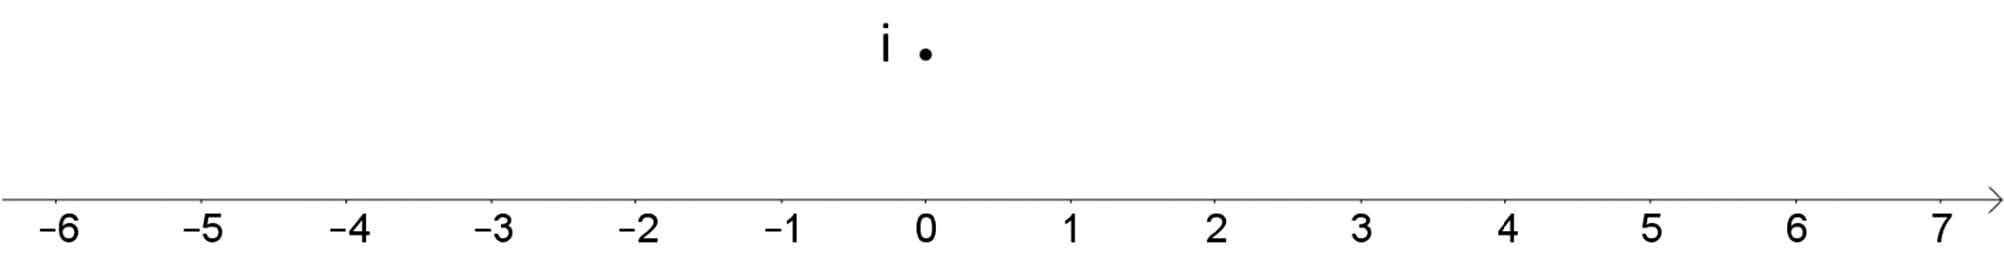
\includegraphics[width = 0.9 \textwidth]{media/Zahlengeradei.jpg}
% \end{center}

Wenn man diese Idee auf alle anderen komplexen Zahlen überträgt, erhält man die \textit{komplexe Zahlenebene} oder \textit{Gauss'sche Zahlenebene:}

\begin{center}
    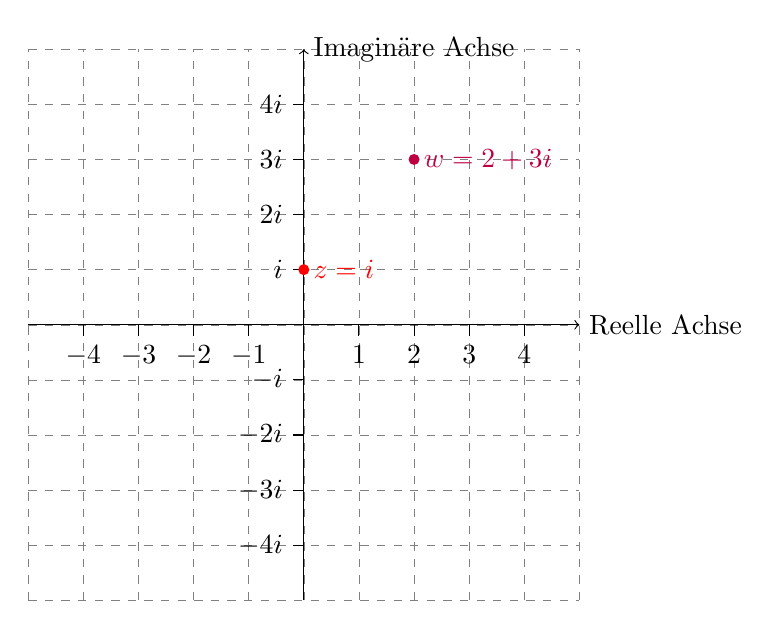
\begin{tikzpicture}[scale=0.7]
        % Gitter
        \draw[dashed, very thin, gray] (-5,-5) grid (5,5);
        
        % Achsen mit Skala
        \draw[->] (-5,0) -- (5,0) node[right] {Reelle Achse};
        \draw[->] (0,-5) -- (0,5) node[right] {Imaginäre Achse};
        \foreach \x in {-4,-3,-2,-1,1,2,3,4} 
            \draw (\x,0) -- (\x,-0.2) node[below] {$\x$};
         \foreach \y in {-4,-3,-2,2,3,4}
            \draw (0,\y) -- (-0.2,\y) node[left] {$\y i$};
        \draw (0,1) -- (-0.2,1) node[left] {$i$};
        \draw (0,-1) -- (-0.2,-1) node[left] {$-i$};
        
        % Punkte und Markierungen
        %\draw[dashed, very thin, gray] (2,0) -- (2,3) -- (0,3);
        \fill[red] (0,1) circle (0.1) node[right] {$z = i$};
        \fill[purple] (2,3) circle (0.1) node[right] {$w = 2 + 3i$};
    \end{tikzpicture}
\end{center}

\clearpage
\begin{ueb}
    {Zur komplexen Zahlenebene}{}
   \begin{enumerate}
    \item Stellen Sie die nachfolgenden komplexen Zahlen in der Gauss'schen Zahlenebene dar:
    \begin{multicols}{3}
    \begin{enumerate}
        \item $2$
        \item $3i$
        \item $-2$
        \item $-4-2i$
        \item $-4+2i$
        \item $4+2i$
    \end{enumerate}
\end{multicols}
    \begin{center}
        
            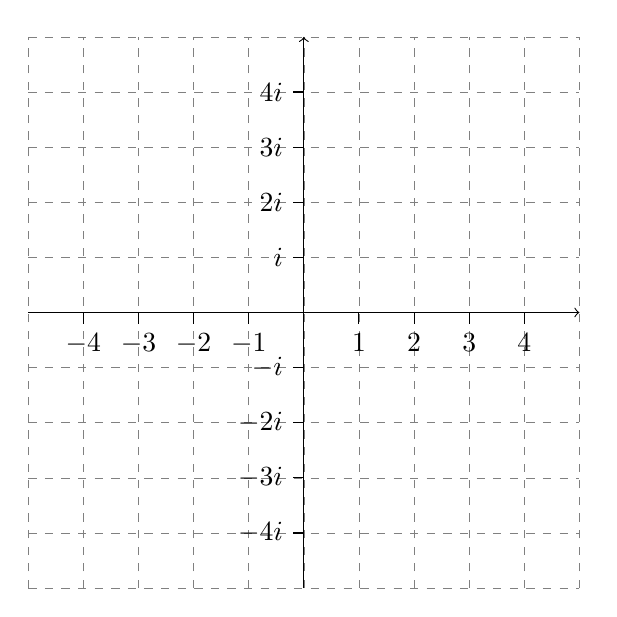
\begin{tikzpicture}[scale = 0.7]
                % Gitter
                \draw[dashed, very thin, gray] (-5,-5) grid (5,5);
                
                % Achsen mit Skala
                \draw[->] (-5,0) -- (5,0) node[above] {$\RE$};
                \draw[->] (0,-5) -- (0,5) node[right] {$\IM$};
                \foreach \x in {-4,-3,-2,-1,1,2,3,4} 
                    \draw (\x,0) -- (\x,-0.2) node[below] {$\x$};
                 \foreach \y in {-4,-3,-2,2,3,4}
                    \draw (0,\y) -- (-0.2,\y) node[left] {$\y i$};
                \draw (0,1) -- (-0.2,1) node[left] {$i$};
                \draw (0,-1) -- (-0.2,-1) node[left] {$-i$};
                
                % Punkte und Markierungen
                % \draw[dashed, very thin, gray] (2,0) -- (2,3) -- (0,3);
                % \fill[red] (0,1) circle (0.1) node[right] {$z = i$};
                % \fill[purple] (2,3) circle (0.1) node[right] {$w = 2 + 3i$};
            \end{tikzpicture}
        \end{center}
    \item     Gegeben ist die komplexe Zahl $z=3+2i$. Stellen Sie die nachfolgenden komplexen Zahlen in der Gauss'schen Zahlenebene dar:
        \begin{multicols}{3}
        \begin{enumerate}
            \item $z$
            \item $-z$
            \item $\overline{z}$
            \item $-\overline{z}$
            \item $i\cdot z$
            \item $\frac{z}{i}$
        \end{enumerate}
    \end{multicols}
    \begin{center}
        
        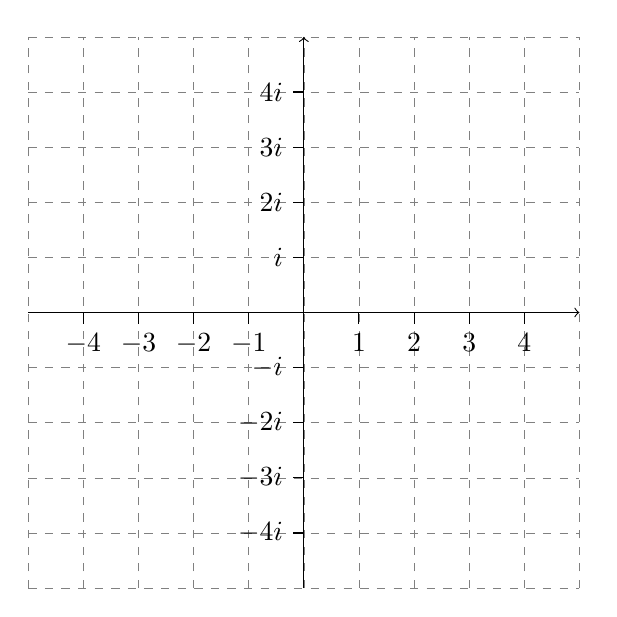
\begin{tikzpicture}[scale = 0.7]
            % Gitter
            \draw[dashed, very thin, gray] (-5,-5) grid (5,5);
            
            % Achsen mit Skala
            \draw[->] (-5,0) -- (5,0) node[above] {$\RE$};
            \draw[->] (0,-5) -- (0,5) node[right] {$\IM$};
            \foreach \x in {-4,-3,-2,-1,1,2,3,4} 
                \draw (\x,0) -- (\x,-0.2) node[below] {$\x$};
             \foreach \y in {-4,-3,-2,2,3,4}
                \draw (0,\y) -- (-0.2,\y) node[left] {$\y i$};
            \draw (0,1) -- (-0.2,1) node[left] {$i$};
            \draw (0,-1) -- (-0.2,-1) node[left] {$-i$};
            
            % Punkte und Markierungen
            % \draw[dashed, very thin, gray] (2,0) -- (2,3) -- (0,3);
            % \fill[red] (0,1) circle (0.1) node[right] {$z = i$};
            % \fill[purple] (2,3) circle (0.1) node[right] {$w = 2 + 3i$};
        \end{tikzpicture}
    \end{center}
       
\newpage
\item Markieren Sie in der Zahlenebene die Menge aller Zahlen mit der angegebenen Eigenschaft:
        \begin{multicols}{2}
            \begin{enumerate}
                \item[\textbf{a)}] Der Imaginärteil ist 2.
                \begin{center}
        
                    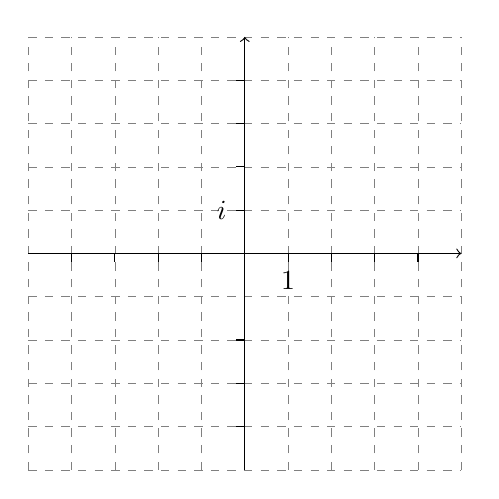
\begin{tikzpicture}[scale = 0.55]
                        % Gitter
                        \draw[dashed, very thin, gray] (-5,-5) grid (5,5);
                        
                        % Achsen mit Skala
                        \draw[->] (-5,0) -- (5,0) node[above] {$\RE$};
                        \draw[->] (0,-5) -- (0,5) node[right] {$\IM$};
                        \foreach \x in {-4,-3,-2,-1,1,2,3,4} 
                            \draw (\x,0) -- (\x,-0.2) ;
                         \foreach \y in {-4,-3,-2,2,3,4}
                            \draw (0,\y) -- (-0.2,\y) ;
                        \draw (0,1) -- (-0.2,1) node[left] {$i$};
                        \draw (1,0) -- (1,-0.2) node[below] {$1$};
                        
                        % Punkte und Markierungen
                        % \draw[dashed, very thin, gray] (2,0) -- (2,3) -- (0,3);
                        % \fill[red] (0,1) circle (0.1) node[right] {$z = i$};
                        % \fill[purple] (2,3) circle (0.1) node[right] {$w = 2 + 3i$};
                    \end{tikzpicture}
                \end{center}
                
                \item[\textbf{b)}] $-1 \leq \operatorname{Re}(z) < 4$
                \begin{center}
        
                    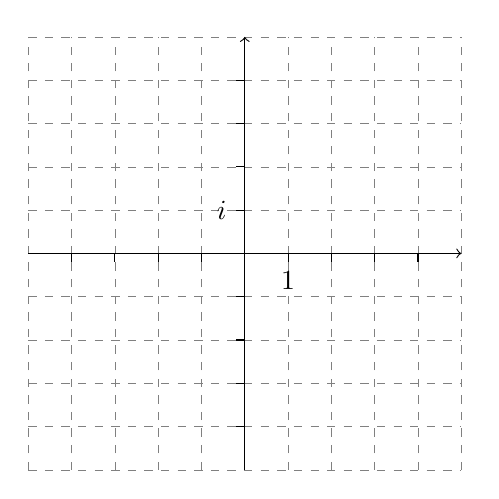
\begin{tikzpicture}[scale = 0.55]
                        % Gitter
                        \draw[dashed, very thin, gray] (-5,-5) grid (5,5);
                        
                        % Achsen mit Skala
                        \draw[->] (-5,0) -- (5,0) node[above] {$\RE$};
                        \draw[->] (0,-5) -- (0,5) node[right] {$\IM$};
                        \foreach \x in {-4,-3,-2,-1,1,2,3,4} 
                            \draw (\x,0) -- (\x,-0.2) ;
                         \foreach \y in {-4,-3,-2, -1,2,3,4}
                            \draw (0,\y) -- (-0.2,\y) ;
                        \draw (0,1) -- (-0.2,1) node[left] {$i$};
                        \draw (1,0) -- (1,-0.2) node[below] {$1$};
                        
                        % Punkte und Markierungen
                        % \draw[dashed, very thin, gray] (2,0) -- (2,3) -- (0,3);
                        % \fill[red] (0,1) circle (0.1) node[right] {$z = i$};
                        % \fill[purple] (2,3) circle (0.1) node[right] {$w = 2 + 3i$};
                    \end{tikzpicture}
                \end{center}
                
                
                
                \item[\textbf{c)}] $\operatorname{Re}(z)^2 + \operatorname{Im}(z)^2 = 4$
                \begin{center}
        
                    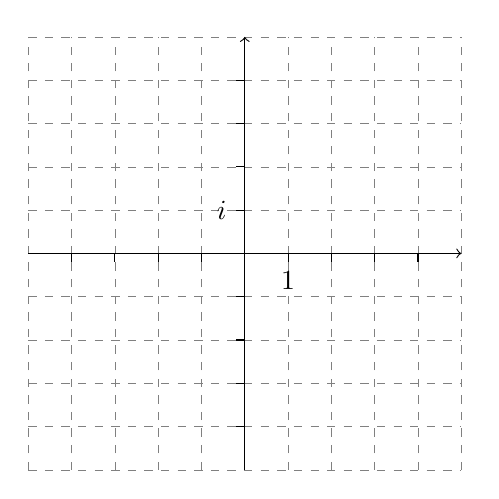
\begin{tikzpicture}[scale = 0.55]
                        % Gitter
                        \draw[dashed, very thin, gray] (-5,-5) grid (5,5);
                        
                        % Achsen mit Skala
                        \draw[->] (-5,0) -- (5,0) node[above] {$\RE$};
                        \draw[->] (0,-5) -- (0,5) node[right] {$\IM$};
                        \foreach \x in {-4,-3,-2,-1,1,2,3,4} 
                            \draw (\x,0) -- (\x,-0.2) ;
                         \foreach \y in {-4,-3,-2, -1,2,3,4}
                            \draw (0,\y) -- (-0.2,\y) ;
                        \draw (0,1) -- (-0.2,1) node[left] {$i$};
                        \draw (1,0) -- (1,-0.2) node[below] {$1$};
                        
                        % Punkte und Markierungen
                        % \draw[dashed, very thin, gray] (2,0) -- (2,3) -- (0,3);
                        % \fill[red] (0,1) circle (0.1) node[right] {$z = i$};
                        % \fill[purple] (2,3) circle (0.1) node[right] {$w = 2 + 3i$};
                    \end{tikzpicture}
                \end{center}
                
                
                \item[\textbf{d)}] $\operatorname{Re}(z) = 2 \cdot \operatorname{Im}(z)$
                \begin{center}
        
                    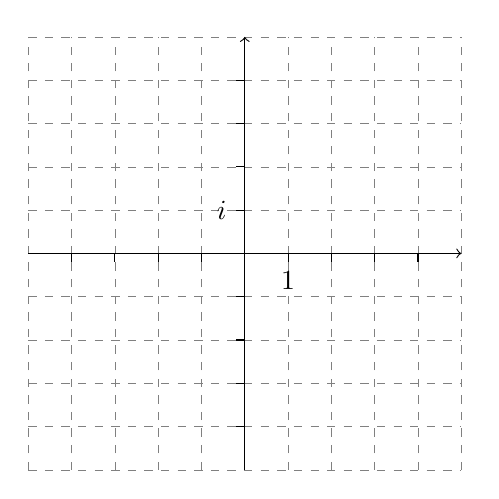
\begin{tikzpicture}[scale = 0.55]
                        % Gitter
                        \draw[dashed, very thin, gray] (-5,-5) grid (5,5);
                        
                        % Achsen mit Skala
                        \draw[->] (-5,0) -- (5,0) node[above] {$\RE$};
                        \draw[->] (0,-5) -- (0,5) node[right] {$\IM$};
                        \foreach \x in {-4,-3,-2,-1,1,2,3,4} 
                            \draw (\x,0) -- (\x,-0.2) ;
                         \foreach \y in {-4,-3,-2, -1,2,3,4}
                            \draw (0,\y) -- (-0.2,\y) ;
                        \draw (0,1) -- (-0.2,1) node[left] {$i$};
                        \draw (1,0) -- (1,-0.2) node[below] {$1$};
                        
                        % Punkte und Markierungen
                        % \draw[dashed, very thin, gray] (2,0) -- (2,3) -- (0,3);
                        % \fill[red] (0,1) circle (0.1) node[right] {$z = i$};
                        % \fill[purple] (2,3) circle (0.1) node[right] {$w = 2 + 3i$};
                    \end{tikzpicture}
                \end{center}
                
                
                \item[\textbf{e)}] $\operatorname{Im}(\bar{z}) \geq 1$
                \begin{center}
        
                    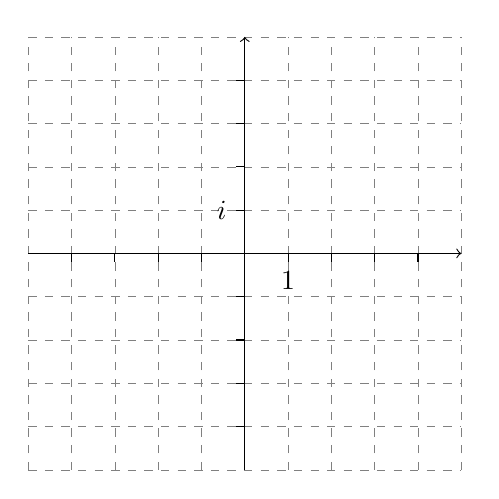
\begin{tikzpicture}[scale = 0.55]
                        % Gitter
                        \draw[dashed, very thin, gray] (-5,-5) grid (5,5);
                        
                        % Achsen mit Skala
                        \draw[->] (-5,0) -- (5,0) node[above] {$\RE$};
                        \draw[->] (0,-5) -- (0,5) node[right] {$\IM$};
                        \foreach \x in {-4,-3,-2,-1,1,2,3,4} 
                            \draw (\x,0) -- (\x,-0.2) ;
                         \foreach \y in {-4,-3,-2, -1,2,3,4}
                            \draw (0,\y) -- (-0.2,\y) ;
                        \draw (0,1) -- (-0.2,1) node[left] {$i$};
                        \draw (1,0) -- (1,-0.2) node[below] {$1$};
                        
                        % Punkte und Markierungen
                        % \draw[dashed, very thin, gray] (2,0) -- (2,3) -- (0,3);
                        % \fill[red] (0,1) circle (0.1) node[right] {$z = i$};
                        % \fill[purple] (2,3) circle (0.1) node[right] {$w = 2 + 3i$};
                    \end{tikzpicture}
                \end{center}
                
                
                
                \item[\textbf{f)}] $(\operatorname{Re}(z) + \operatorname{Im}(z))^2 = 1$
                \begin{center}
        
                    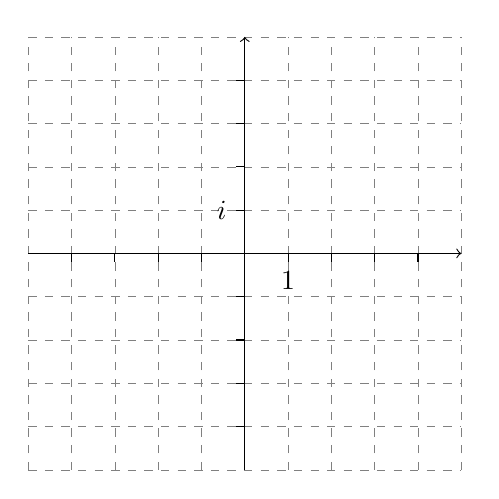
\begin{tikzpicture}[scale = 0.55]
                        % Gitter
                        \draw[dashed, very thin, gray] (-5,-5) grid (5,5);
                        
                        % Achsen mit Skala
                        \draw[->] (-5,0) -- (5,0) node[above] {$\RE$};
                        \draw[->] (0,-5) -- (0,5) node[right] {$\IM$};
                        \foreach \x in {-4,-3,-2,-1,1,2,3,4} 
                            \draw (\x,0) -- (\x,-0.2) ;
                         \foreach \y in {-4,-3,-2, -1,2,3,4}
                            \draw (0,\y) -- (-0.2,\y) ;
                        \draw (0,1) -- (-0.2,1) node[left] {$i$};
                        \draw (1,0) -- (1,-0.2) node[below] {$1$};
                        
                        % Punkte und Markierungen
                        % \draw[dashed, very thin, gray] (2,0) -- (2,3) -- (0,3);
                        % \fill[red] (0,1) circle (0.1) node[right] {$z = i$};
                        % \fill[purple] (2,3) circle (0.1) node[right] {$w = 2 + 3i$};
                    \end{tikzpicture}
                \end{center}
                
                
            \end{enumerate}
            \end{multicols}
        \end{enumerate}
            
\end{ueb}


\clearpage
\emph{Lösungen}
\begin{enumerate}
    \item Stellen Sie die nachfolgenden komplexen Zahlen in der Gauss'schen Zahlenebene dar:
      \begin{center}
        
            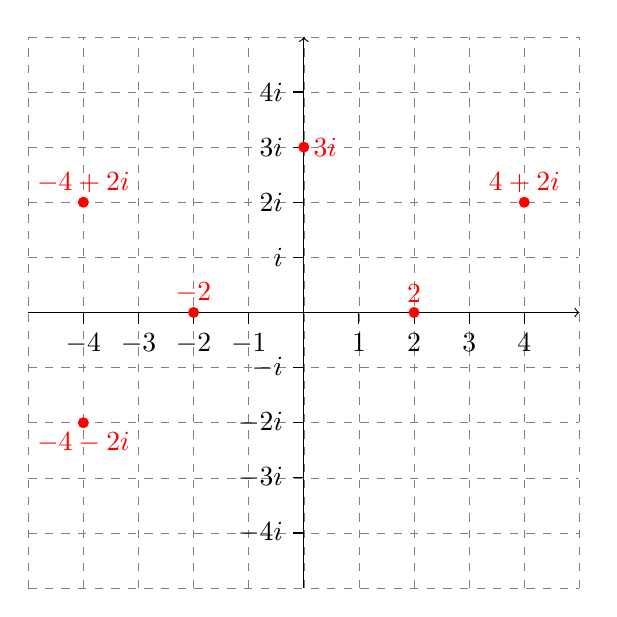
\begin{tikzpicture}[scale = 0.7]
                % Gitter
                \draw[dashed, very thin, gray] (-5,-5) grid (5,5);
                
                % Achsen mit Skala
                \draw[->] (-5,0) -- (5,0) node[above] {$\RE$};
                \draw[->] (0,-5) -- (0,5) node[right] {$\IM$};
                \foreach \x in {-4,-3,-2,-1,1,2,3,4} 
                    \draw (\x,0) -- (\x,-0.2) node[below] {$\x$};
                 \foreach \y in {-4,-3,-2,2,3,4}
                    \draw (0,\y) -- (-0.2,\y) node[left] {$\y i$};
                \draw (0,1) -- (-0.2,1) node[left] {$i$};
                \draw (0,-1) -- (-0.2,-1) node[left] {$-i$};
                
                % Punkte und Markierungen
                \fill[red] (2,0) circle (0.1) node[above] {$2$};
                \fill[red] (0,3) circle (0.1) node[right] {$3i$};
                \fill[red] (-2,0) circle (0.1) node[above] {$-2$};
                \fill[red] (-4,-2) circle (0.1) node[below] {$-4-2i$};
                \fill[red] (-4,2) circle (0.1) node[above] {$-4+2i$};
                \fill[red] (4,2) circle (0.1) node[above] {$4+2i$};
            \end{tikzpicture}
        \end{center}
    \item     Gegeben ist die komplexe Zahl $z=3+2i$. Stellen Sie die nachfolgenden komplexen Zahlen in der Gauss'schen Zahlenebene dar:
        
    \begin{center}
        
        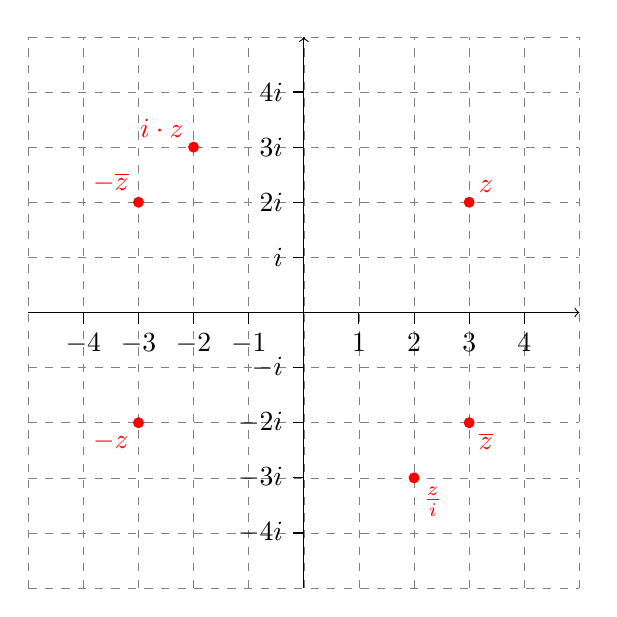
\begin{tikzpicture}[scale = 0.7]
            % Gitter
            \draw[dashed, very thin, gray] (-5,-5) grid (5,5);
            
            % Achsen mit Skala
            \draw[->] (-5,0) -- (5,0) node[above] {$\RE$};
            \draw[->] (0,-5) -- (0,5) node[right] {$\IM$};
            \foreach \x in {-4,-3,-2,-1,1,2,3,4} 
                \draw (\x,0) -- (\x,-0.2) node[below] {$\x$};
             \foreach \y in {-4,-3,-2,2,3,4}
                \draw (0,\y) -- (-0.2,\y) node[left] {$\y i$};
            \draw (0,1) -- (-0.2,1) node[left] {$i$};
            \draw (0,-1) -- (-0.2,-1) node[left] {$-i$};
            
            % Punkte und Markierungen
            \fill[red] (3,2) circle (0.1) node[above right] {$z$};
            \fill[red] (-3,-2) circle (0.1) node[below left] {$-z$};
            \fill[red] (3,-2) circle (0.1) node[below right] {$\overline{z}$};
            \fill[red] (-3,2) circle (0.1) node[above left] {$-\overline{z}$};
            \fill[red] (-2,3) circle (0.1) node[above left] {$i \cdot z$};
            \fill[red] (2,-3) circle (0.1) node[below right] {$\frac{z}{i}$};
        \end{tikzpicture}
    \end{center}
       
\newpage
\item Markieren Sie in der Zahlenebene die Menge aller Zahlen mit der angegebenen Eigenschaft:
        \begin{multicols}{2}
            \begin{enumerate}
                \item[\textbf{a)}] Der Imaginärteil ist 2.
                \begin{center}
        
                    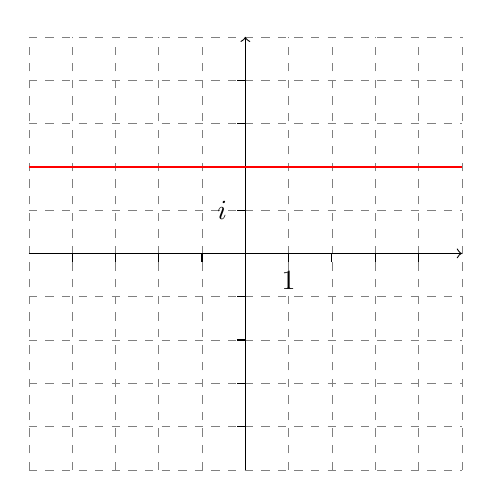
\begin{tikzpicture}[scale = 0.55]
                        % Gitter
                        \draw[dashed, very thin, gray] (-5,-5) grid (5,5);
                        
                        % Achsen mit Skala
                        \draw[->] (-5,0) -- (5,0) node[above] {$\RE$};
                        \draw[->] (0,-5) -- (0,5) node[right] {$\IM$};
                        \foreach \x in {-4,-3,-2,-1,1,2,3,4} 
                            \draw (\x,0) -- (\x,-0.2) ;
                         \foreach \y in {-4,-3,-2, -1,2,3,4}
                            \draw (0,\y) -- (-0.2,\y) ;
                        \draw (0,1) -- (-0.2,1) node[left] {$i$};
                        \draw (1,0) -- (1,-0.2) node[below] {$1$};
                        
                        % Punkte und Markierungen
                        \draw[thick, red] (-5,2) -- (5,2);
            
                    \end{tikzpicture}
                \end{center}
                
                \item[\textbf{b)}] $-1 \leq \operatorname{Re}(z) < 4$
                \begin{center}
        
                    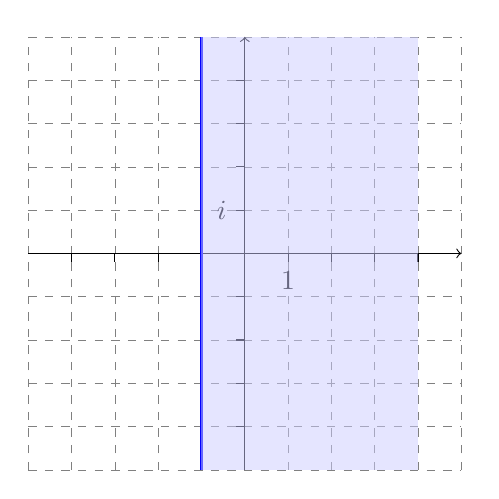
\begin{tikzpicture}[scale = 0.55]
                        % Gitter
                        \draw[dashed, very thin, gray] (-5,-5) grid (5,5);
                        
                        % Achsen mit Skala
                        \draw[->] (-5,0) -- (5,0) node[above] {$\RE$};
                        \draw[->] (0,-5) -- (0,5) node[right] {$\IM$};
                        \foreach \x in {-4,-3,-2,-1,1,2,3,4} 
                            \draw (\x,0) -- (\x,-0.2) ;
                         \foreach \y in {-4,-3,-2, -1,2,3,4}
                            \draw (0,\y) -- (-0.2,\y) ;
                        \draw (0,1) -- (-0.2,1) node[left] {$i$};
                        \draw (1,0) -- (1,-0.2) node[below] {$1$};
                        
                        % Punkte und Markierungen
                        \draw[thick, blue] (-1,-5) -- (-1,5);
                        %\draw[thick, blue] (4,-5) -- (4,5);
                        \fill[blue!20, opacity=0.5] (-1,-5) -- (-1,5) -- (4,5) -- (4,-5) -- cycle;
                    \end{tikzpicture}
                \end{center}
                
                
                
                \item[\textbf{c)}] $\operatorname{Re}(z)^2 + \operatorname{Im}(z)^2 = 4$
                \begin{center}
        
                    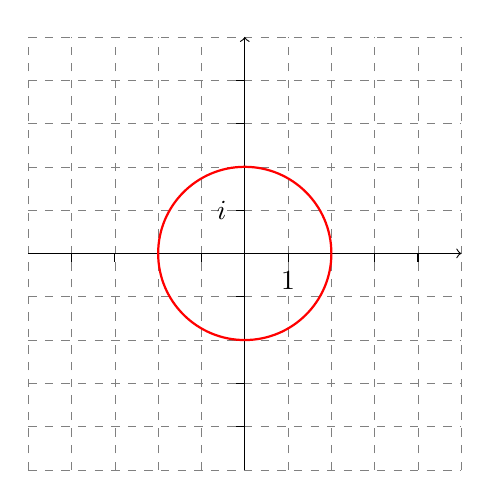
\begin{tikzpicture}[scale = 0.55]
                        % Gitter
                        \draw[dashed, very thin, gray] (-5,-5) grid (5,5);
                        
                        % Achsen mit Skala
                        \draw[->] (-5,0) -- (5,0) node[above] {$\RE$};
                        \draw[->] (0,-5) -- (0,5) node[right] {$\IM$};
                        \foreach \x in {-4,-3,-2,-1,1,2,3,4} 
                            \draw (\x,0) -- (\x,-0.2) ;
                         \foreach \y in {-4,-3,-2, -1,2,3,4}
                            \draw (0,\y) -- (-0.2,\y) ;
                        \draw (0,1) -- (-0.2,1) node[left] {$i$};
                        \draw (1,0) -- (1,-0.2) node[below] {$1$};
                        
                        % Punkte und Markierungen
                        \draw[thick, red] (0,0) circle (2);
            
                    \end{tikzpicture}
                \end{center}
                
                
                \item[\textbf{d)}] $\operatorname{Re}(z) = 2 \cdot \operatorname{Im}(z)$
                \begin{center}
        
                    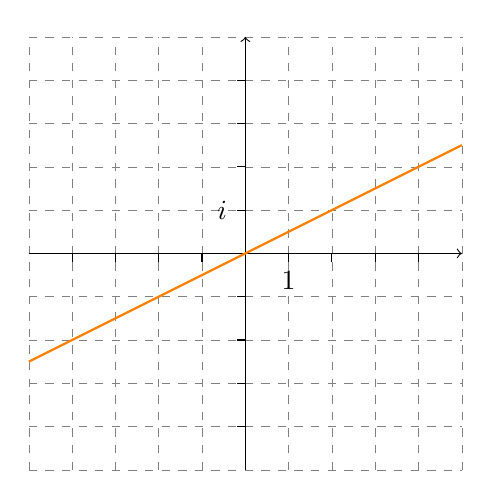
\begin{tikzpicture}[scale = 0.55]
                        % Gitter
                        \draw[dashed, very thin, gray] (-5,-5) grid (5,5);
                        
                        % Achsen mit Skala
                        \draw[->] (-5,0) -- (5,0) node[above] {$\RE$};
                        \draw[->] (0,-5) -- (0,5) node[right] {$\IM$};
                        \foreach \x in {-4,-3,-2,-1,1,2,3,4} 
                            \draw (\x,0) -- (\x,-0.2) ;
                         \foreach \y in {-4,-3,-2, -1,2,3,4}
                            \draw (0,\y) -- (-0.2,\y) ;
                        \draw (0,1) -- (-0.2,1) node[left] {$i$};
                        \draw (1,0) -- (1,-0.2) node[below] {$1$};
                        
                        % Punkte und Markierungen
                        \draw[thick, orange] (-5,-2.5) -- (5,2.5);
                    \end{tikzpicture}
                \end{center}
                
                
                \item[\textbf{e)}] $\operatorname{Im}(\bar{z}) \geq 1$
                \begin{center}
        
                    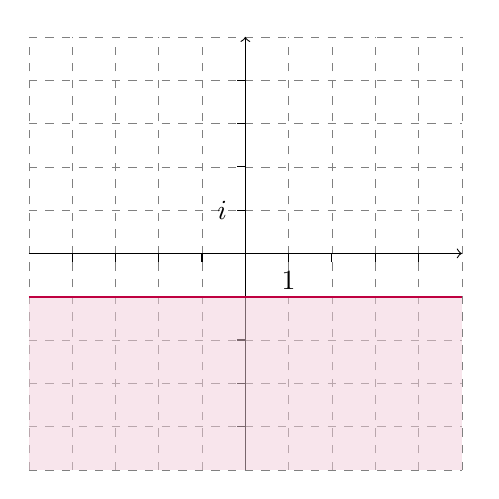
\begin{tikzpicture}[scale = 0.55]
                        % Gitter
                        \draw[dashed, very thin, gray] (-5,-5) grid (5,5);
                        
                        % Achsen mit Skala
                        \draw[->] (-5,0) -- (5,0) node[above] {$\RE$};
                        \draw[->] (0,-5) -- (0,5) node[right] {$\IM$};
                        \foreach \x in {-4,-3,-2,-1,1,2,3,4} 
                            \draw (\x,0) -- (\x,-0.2) ;
                         \foreach \y in {-4,-3,-2, -1,2,3,4}
                            \draw (0,\y) -- (-0.2,\y) ;
                        \draw (0,1) -- (-0.2,1) node[left] {$i$};
                        \draw (1,0) -- (1,-0.2) node[below] {$1$};
                        
                        % Punkte und Markierungen
                        %\draw[thick, purple] (-5,-1) -- (5,-1);
                        \fill[purple!20, opacity=0.5] (-5,-1) -- (5,-1) -- (5,-5) -- (-5,-5) -- cycle;
                        \draw[thick, purple] (-5,-1) -- (5,-1);
                    \end{tikzpicture}
                \end{center}
                
                
                
                \item[\textbf{f)}] $(\operatorname{Re}(z) + \operatorname{Im}(z))^2 = 1$
                \begin{center}
        
                    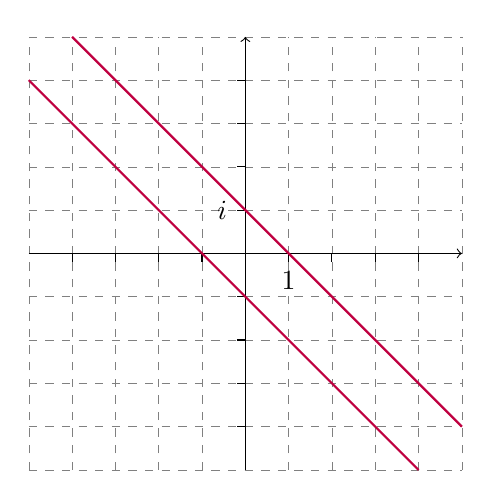
\begin{tikzpicture}[scale = 0.55]
                        % Gitter
                        \draw[dashed, very thin, gray] (-5,-5) grid (5,5);
                        
                        % Achsen mit Skala
                        \draw[->] (-5,0) -- (5,0) node[above] {$\RE$};
                        \draw[->] (0,-5) -- (0,5) node[right] {$\IM$};
                        \foreach \x in {-4,-3,-2,-1,1,2,3,4} 
                            \draw (\x,0) -- (\x,-0.2) ;
                         \foreach \y in {-4,-3,-2, -1,2,3,4}
                            \draw (0,\y) -- (-0.2,\y) ;
                        \draw (0,1) -- (-0.2,1) node[left] {$i$};
                        \draw (1,0) -- (1,-0.2) node[below] {$1$};
                        
                        % Punkte und Markierungen
                        \draw[thick, purple] (-5,4) -- (4,-5);
                        \draw[thick, purple] (-4,5) -- (5,-4);
                    \end{tikzpicture}
                \end{center}
                
                
            \end{enumerate}
            \end{multicols}
        \end{enumerate}
            




















































\clearpage
\subsection{Der Betrag komplexer Zahlen}
Das Konzept des Betrags einer reellen Zahl kann auf komplexe Zahlen erweitert werden, indem der Betrag einer komplexen Zahl als deren Abstand zum Ursprung in der komplexen Zahlenebene definiert wird.
\begin{center}
    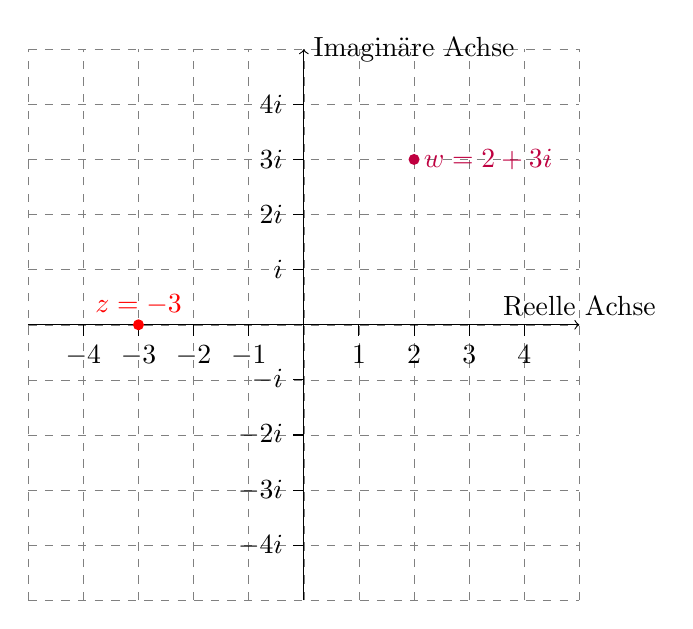
\begin{tikzpicture}[scale = 0.7]
        % Gitter
        \draw[dashed, very thin, very thin, gray] (-5,-5) grid (5,5);
        
        % Achsen mit Skala
        \draw[->] (-5,0) -- (5,0) node[above] {Reelle Achse};
        \draw[->] (0,-5) -- (0,5) node[right] {Imaginäre Achse};
        \foreach \x in {-4,-3,-2,-1,1,2,3,4} 
            \draw (\x,0) -- (\x,-0.2) node[below] {$\x$};
         \foreach \y in {-4,-3,-2,2,3,4}
            \draw (0,\y) -- (-0.2,\y) node[left] {$\y i$};
        \draw (0,1) -- (-0.2,1) node[left] {$i$};
        \draw (0,-1) -- (-0.2,-1) node[left] {$-i$};
        % Punkte und Markierungen
         \fill[red] (-3,0) circle (0.1) node[above] {$z = -3$};
         \fill[purple] (2,3) circle (0.1) node[right] {$w = 2 + 3i$};
    \end{tikzpicture}
\end{center}

\begin{definition}
    {Der Betrag einer komplexen Zahl}{}
    Der \emph{Betrag} einer komplexen Zahl $z=a+bi$ entspricht dem Abstand von $z$ zum Urspung $O(0, 0)$ in der komplexen Zahlenebene. Der Betrag von $z=a+bi$ wird so berechnet: 

$$|z|=|a+bi|=\ldots\ldots$$

\end{definition}

\begin{ueb}
    {}{}
    \begin{enumerate}
        \item  Gegeben sind $v=-3-4i$, $w=-2i$ und $z=1+i$. Berechnen Sie
        \begin{enumerate}
            \item $|z|=$
            \vfill
            \item $|\overline{w}|=$
            \vfill
            \item $|2v|=$
            \vfill
            \item $\left|\frac{v}{z}\right|=$
            \vfill
            \item $\left|w\cdot v\right|=$
            \vfill
        \end{enumerate}
        \item Zeigen Sie, dass für alle $z\in \C$ gilt: $z\cdot \overline{z}=|z|^2$.
        \item Zeigen Sie, dass $|z-w|$ dem Abstand der beiden Zahlen $z$ und $w$ in der komplexe Zahlenebene entspricht.
        \item Markieren Sie in der Gauss'schen Zahlenebene jeweils alle komplexe Zahlen $z$ mit folgender Eigenschaft:

        \begin{multicols}{2}
        \begin{enumerate}
            \item $|z|<3$
            \begin{center}
        
                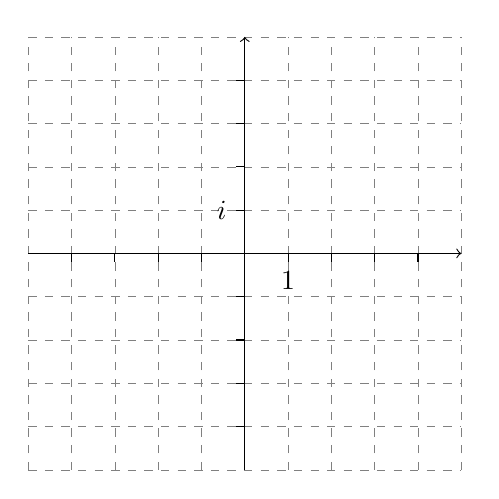
\begin{tikzpicture}[scale = 0.55]
                    % Gitter
                    \draw[dashed, very thin, gray] (-5,-5) grid (5,5);
                    
                    % Achsen mit Skala
                    \draw[->] (-5,0) -- (5,0) node[above] {$\RE$};
                    \draw[->] (0,-5) -- (0,5) node[right] {$\IM$};
                    \foreach \x in {-4,-3,-2,-1,1,2,3,4} 
                        \draw (\x,0) -- (\x,-0.2) ;
                     \foreach \y in {-4,-3,-2, -1,2,3,4}
                        \draw (0,\y) -- (-0.2,\y) ;
                    \draw (0,1) -- (-0.2,1) node[left] {$i$};
                    \draw (1,0) -- (1,-0.2) node[below] {$1$};
                    
                    % Punkte und Markierungen
                    % \draw[dashed, very thin, gray] (2,0) -- (2,3) -- (0,3);
                    % \fill[red] (0,1) circle (0.1) node[right] {$z = i$};
                    % \fill[purple] (2,3) circle (0.1) node[right] {$w = 2 + 3i$};
                \end{tikzpicture}
            \end{center}
            
            \item $\IM(z)=|z|$
            \begin{center}
        
                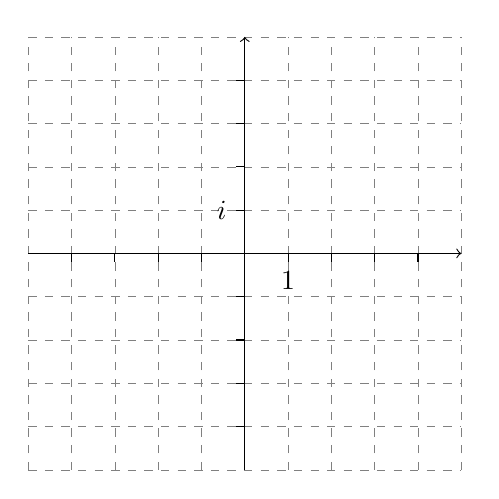
\begin{tikzpicture}[scale = 0.55]
                    % Gitter
                    \draw[dashed, very thin, gray] (-5,-5) grid (5,5);
                    
                    % Achsen mit Skala
                    \draw[->] (-5,0) -- (5,0) node[above] {$\RE$};
                    \draw[->] (0,-5) -- (0,5) node[right] {$\IM$};
                    \foreach \x in {-4,-3,-2,-1,1,2,3,4} 
                        \draw (\x,0) -- (\x,-0.2) ;
                     \foreach \y in {-4,-3,-2, -1,2,3,4}
                        \draw (0,\y) -- (-0.2,\y) ;
                    \draw (0,1) -- (-0.2,1) node[left] {$i$};
                    \draw (1,0) -- (1,-0.2) node[below] {$1$};
                    
                    % Punkte und Markierungen
                    % \draw[dashed, very thin, gray] (2,0) -- (2,3) -- (0,3);
                    % \fill[red] (0,1) circle (0.1) node[right] {$z = i$};
                    % \fill[purple] (2,3) circle (0.1) node[right] {$w = 2 + 3i$};
                \end{tikzpicture}
            
            \end{center}

            \item $|z- 3| = 2$
            \begin{center}
        
                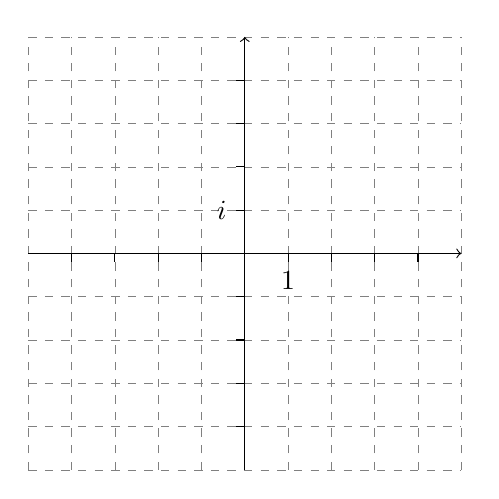
\begin{tikzpicture}[scale = 0.55]
                    % Gitter
                    \draw[dashed, very thin, gray] (-5,-5) grid (5,5);
                    
                    % Achsen mit Skala
                    \draw[->] (-5,0) -- (5,0) node[above] {$\RE$};
                    \draw[->] (0,-5) -- (0,5) node[right] {$\IM$};
                    \foreach \x in {-4,-3,-2,-1,1,2,3,4} 
                        \draw (\x,0) -- (\x,-0.2) ;
                     \foreach \y in {-4,-3,-2, -1,2,3,4}
                        \draw (0,\y) -- (-0.2,\y) ;
                    \draw (0,1) -- (-0.2,1) node[left] {$i$};
                    \draw (1,0) -- (1,-0.2) node[below] {$1$};
                    
                    % Punkte und Markierungen
                    % \draw[dashed, very thin, gray] (2,0) -- (2,3) -- (0,3);
                    % \fill[red] (0,1) circle (0.1) node[right] {$z = i$};
                    % \fill[purple] (2,3) circle (0.1) node[right] {$w = 2 + 3i$};
                \end{tikzpicture}
            \end{center}

            
            \item $|z+i|\geq 2$
            \begin{center}
        
                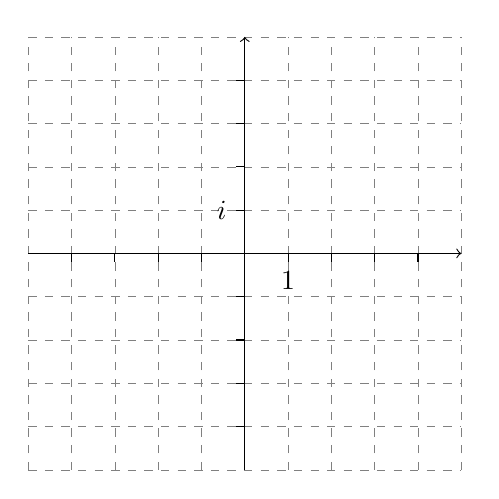
\begin{tikzpicture}[scale = 0.55]
                    % Gitter
                    \draw[dashed, very thin, gray] (-5,-5) grid (5,5);
                    
                    % Achsen mit Skala
                    \draw[->] (-5,0) -- (5,0) node[above] {$\RE$};
                    \draw[->] (0,-5) -- (0,5) node[right] {$\IM$};
                    \foreach \x in {-4,-3,-2,-1,1,2,3,4} 
                        \draw (\x,0) -- (\x,-0.2) ;
                     \foreach \y in {-4,-3,-2, -1,2,3,4}
                        \draw (0,\y) -- (-0.2,\y) ;
                    \draw (0,1) -- (-0.2,1) node[left] {$i$};
                    \draw (1,0) -- (1,-0.2) node[below] {$1$};
                    
                    % Punkte und Markierungen
                    % \draw[dashed, very thin, gray] (2,0) -- (2,3) -- (0,3);
                    % \fill[red] (0,1) circle (0.1) node[right] {$z = i$};
                    % \fill[purple] (2,3) circle (0.1) node[right] {$w = 2 + 3i$};
                \end{tikzpicture}
            \end{center}
            
        \end{enumerate}
        \end{multicols}
        \item Sind die folgenden Aussagen wahr oder falsch? Begründen Sie:

        \begin{enumerate}
            \item Für alle $w,z\in \C$ gilt: $|w\cdot z|=|w|\cdot |z|$.
            \vfill
            \item Für alle $w,z\in \C$ gilt: $|w + z|=|w|+|z|$.
            \vfill
            \item Für alle $z\in \C$ gilt: $|z|=|\overline{z}|$.
            \vfill
        \end{enumerate}
        
    \end{enumerate}
\end{ueb}


\begin{ueb}
    {Programmieraufgabe}{}
    Ergänzen Sie den Konstruktor \lstinline{__init__()} der Klasse `komplex' um das Attribut \lstinline{self.betrag}, worin der Betrag der komplexen Zahl gespeichert wird, sodass man mit \lstinline{z.betrag} den Betrag der Zahl $z$ erhält.



    Für die Berechnung der Wurzel müssen Sie die entsprechende Funktion zuerst importieren: \lstinline{from math import sqrt}
\end{ueb}


\clearpage
\emph{Lösungen}
\begin{enumerate}

\item Gegeben sind $v=-3-4i$, $w=-2i$ und $z=1+i$. Berechnen Sie:
    \begin{enumerate}
        \item $|z|= \sqrt{2}$
        \item $|\overline{w}|= 2$
        \item $|2v|= 10$
        \item $\left|\frac{v}{z}\right|= \frac{5\sqrt{2}}{2}$
        \item $\left|w\cdot v\right|= 10$
    \end{enumerate}
    
    \item  $z\cdot \overline{z}= (a+bi)(a-bi) = a^2+b^2 = |z|^2$.
    
    \item Rechne $|z-w|= |(a+bi)-(c+di)| = \cdots = \sqrt{(a-c)^2+(b-d)^2}$. Vergleiche mit der Berechnung des Abstands der beiden Punkte mit Pythagoras.
    \item Markieren Sie in der Gauss'schen Zahlenebene jeweils alle komplexe Zahlen $z$ mit folgender Eigenschaft:

        \begin{multicols}{2}
        \begin{enumerate}
            \item $|z|<3$
            \begin{center}
        
                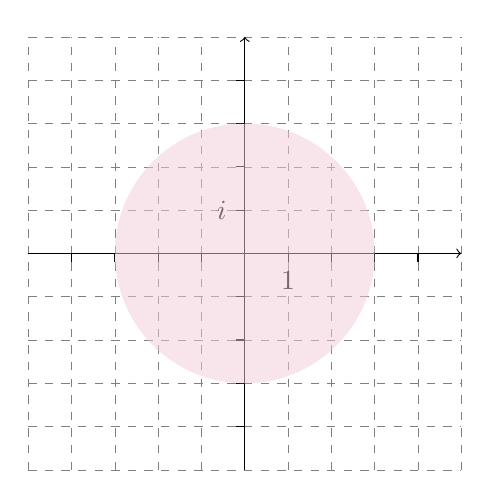
\begin{tikzpicture}[scale = 0.55]
                    % Gitter
                    \draw[dashed, very thin, gray] (-5,-5) grid (5,5);
                    
                    % Achsen mit Skala
                    \draw[->] (-5,0) -- (5,0) node[above] {$\RE$};
                    \draw[->] (0,-5) -- (0,5) node[right] {$\IM$};
                    \foreach \x in {-4,-3,-2,-1,1,2,3,4} 
                        \draw (\x,0) -- (\x,-0.2) ;
                     \foreach \y in {-4,-3,-2, -1,2,3,4}
                        \draw (0,\y) -- (-0.2,\y) ;
                    \draw (0,1) -- (-0.2,1) node[left] {$i$};
                    \draw (1,0) -- (1,-0.2) node[below] {$1$};
                    
                    % Punkte und Markierungen
                    \fill[purple!20, opacity=0.5] (0,0) circle (3);
                \end{tikzpicture}
            \end{center}
            
            \item $\IM(z)=|z|$
            \begin{center}
        
                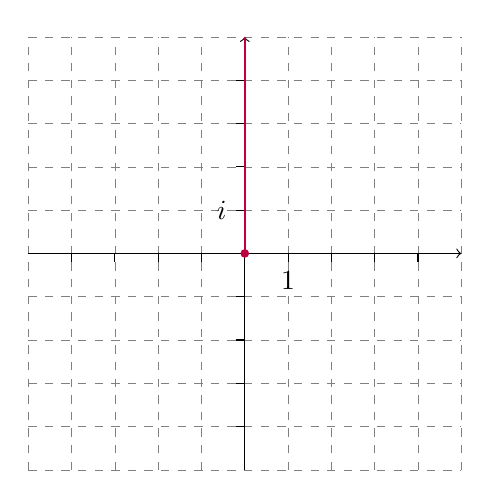
\begin{tikzpicture}[scale = 0.55]
                    % Gitter
                    \draw[dashed, very thin, gray] (-5,-5) grid (5,5);
                    
                    % Achsen mit Skala
                    \draw[->] (-5,0) -- (5,0) node[above] {$\RE$};
                    \draw[->] (0,-5) -- (0,5) node[right] {$\IM$};
                    \foreach \x in {-4,-3,-2,-1,1,2,3,4} 
                        \draw (\x,0) -- (\x,-0.2) ;
                     \foreach \y in {-4,-3,-2, -1,2,3,4}
                        \draw (0,\y) -- (-0.2,\y) ;
                    \draw (0,1) -- (-0.2,1) node[left] {$i$};
                    \draw (1,0) -- (1,-0.2) node[below] {$1$};
                    
                    % Punkte und Markierungen
                    \draw[thick, purple] (0,0) -- (0,5);
                    \fill[purple] (0,0) circle (0.1) ;                    
                \end{tikzpicture}
            
            \end{center}

            \item $|z- 3| = 2$
            \begin{center}
        
                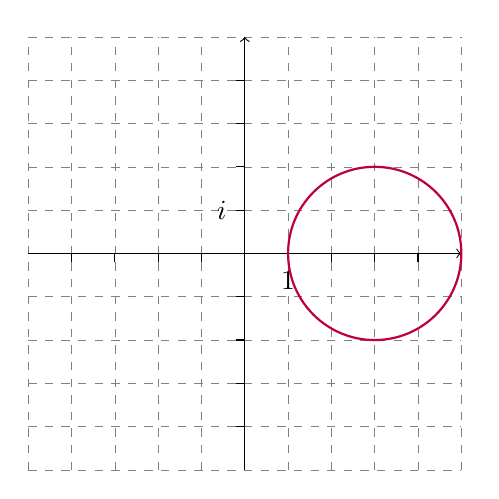
\begin{tikzpicture}[scale = 0.55]
                    % Gitter
                    \draw[dashed, very thin, gray] (-5,-5) grid (5,5);
                    
                    % Achsen mit Skala
                    \draw[->] (-5,0) -- (5,0) node[above] {$\RE$};
                    \draw[->] (0,-5) -- (0,5) node[right] {$\IM$};
                    \foreach \x in {-4,-3,-2,-1,1,2,3,4} 
                        \draw (\x,0) -- (\x,-0.2) ;
                     \foreach \y in {-4,-3,-2, -1,2,3,4}
                        \draw (0,\y) -- (-0.2,\y) ;
                    \draw (0,1) -- (-0.2,1) node[left] {$i$};
                    \draw (1,0) -- (1,-0.2) node[below] {$1$};
                    
                    % Punkte und Markierungen
                    \draw[thick, purple] (3,0) circle (2);
                \end{tikzpicture}
            \end{center}

            
            \item $|z+i|\geq 2$
            \begin{center}
        
                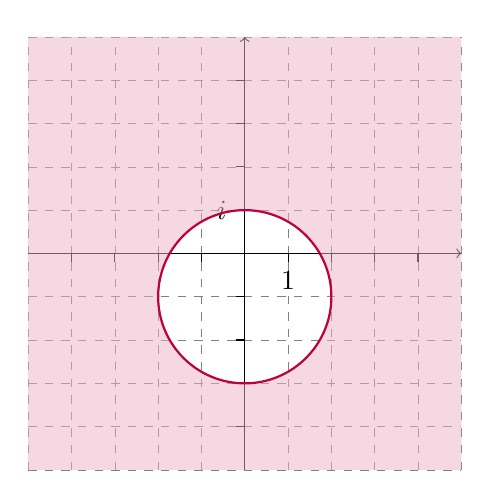
\begin{tikzpicture}[scale = 0.55, even odd rule]
                    % Gitter
                    \draw[dashed, very thin, gray] (-5,-5) grid (5,5);
                    
                    % Achsen mit Skala
                    \draw[->] (-5,0) -- (5,0) node[above] {$\RE$};
                    \draw[->] (0,-5) -- (0,5) node[right] {$\IM$};
                    \foreach \x in {-4,-3,-2,-1,1,2,3,4} 
                        \draw (\x,0) -- (\x,-0.2) ;
                     \foreach \y in {-4,-3,-2, -1,2,3,4}
                        \draw (0,\y) -- (-0.2,\y) ;
                    \draw (0,1) -- (-0.2,1) node[left] {$i$};
                    \draw (1,0) -- (1,-0.2) node[below] {$1$};
                    
                    % % Punkte und Markierungen
                    \fill[even odd rule, purple!30, opacity=0.5] (-5,-5) rectangle (5,5) (0,-1) circle (2);
                    \draw[thick, purple] (0,-1) circle (2);

                \end{tikzpicture}
            \end{center}
            
        \end{enumerate}
        \end{multicols}
        \item Sind die folgenden Aussagen wahr oder falsch? 

        \begin{enumerate}
            \item Für alle $w,z\in \C$ gilt: $|w\cdot z|=|w|\cdot |z|$. Setze $z=a+bi, w=c+di$ und rechne \dots WAHR.
            
            \item Für alle $w,z\in \C$ gilt: $|w + z|=|w|+|z|$. Gegenbeispiel $z=1, w=-1$.
            \item Für alle $z\in \C$ gilt: $|z|=|\overline{z}|$. Setze $z=a+bi$ und rechne \dots WAHR.
        \end{enumerate}
        

\end{enumerate}
















































\clearpage
\subsection{Geometrische Interpretation der Grundoperationen}
Die Summe $z+w$, die Differenz $z-w$ und das Produkt $z\cdot w$ zweier komplexer Zahlen haben in der Gauss'schen Zahlenebene eine elegante geometrische Interpretation. Um diese zu sehen, müssen wir aber zuerst die komplexen Zahlen als Ortsvektoren verstehen.

Genauer: wir interpretieren die komplexe Zahl $z=a+bi$ als den Ortsvektor $\vec{z}=\left(\begin{array}{c}a\\b\\ \end{array}\right)$.

Die Addition, Subtraktion und die reellen Vielfache von komplexen Zahlen entspricht dann der analogen Operation für Vektoren.

\begin{multicols}{2}

    \begin{center}

        Addition

        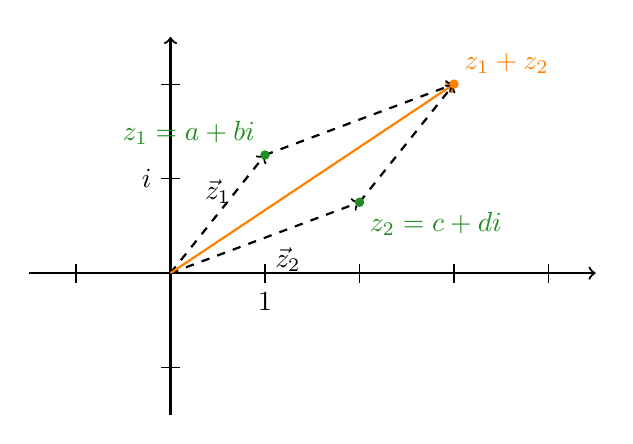
\begin{tikzpicture}[scale = 1.2]
      
            
            % Achsen mit Skala
            \draw[->, thick] (-1.5,0) -- (4.5,0) node[above] {$\RE$};
            \draw[->, thick] (0,-1.5) -- (0,2.5) node[right] {$\IM$};
            \foreach \x in {-1,2,3,4} 
                \draw (\x,0.1) -- (\x,-0.1) ;
            \foreach \y in {-1,2,} 
                \draw (0.1,\y) -- (-0.1,\y) ;
            \draw (0.1,1) -- (-0.1,1) node[left] {$i$};
            \draw (1,0.1) -- (1,-0.1) node[below] {$1$};
            
             % Vektoren
             \draw[->, thick, dashed] (0,0) -- node[above] {$\vec{z}_1$} ++(1,5/4) node[above left, ForestGreen] {$z_1 = a + bi$};
             \draw[->, thick, dashed] (0,0) -- node[below right] {$\vec{z}_2$} ++(2,3/4) node[below right, ForestGreen] {$z_2 = c + di$};
             \draw[->, thick, orange] (0,0) -- (3,2) node[above right, orange] {$z_1 + z_2$};
             \draw[->, thick, dashed] (1,5/4) -- (3,2) ; 
             \draw[->, thick, dashed] (2,3/4) -- (3,2) ; 
            
             % Punkte
             \fill[ForestGreen] (1,5/4) circle (0.05);
             \fill[ForestGreen] (2,3/4) circle (0.05) ;
             \fill[orange] (3,2) circle (0.05);
        \end{tikzpicture}
        
    \end{center}

    \begin{center}
        
        Multiplikation mit einer reellen Zahl

        \begin{tikzpicture}[scale = 1.2]
      
            
            % Achsen mit Skala
            \draw[->, thick] (-1.5,0) -- (4.5,0) node[above] {$\RE$};
            \draw[->, thick] (0,-1.5) -- (0,2.5) node[right] {$\IM$};
            \foreach \x in {-1,2,3,4} 
                \draw (\x,0.1) -- (\x,-0.1) ;
            \foreach \y in {-1,2,} 
                \draw (0.1,\y) -- (-0.1,\y) ;
            \draw (0.1,1) -- (-0.1,1) node[left] {$i$};
            \draw (1,0.1) -- (1,-0.1) node[below] {$1$};
            
             % Vektoren
             \draw[->, very thick] (0,0) -- node[above] {$\vec{z}$} ++(2,1) node[below right, ForestGreen] {$z = a + bi$};
             \draw[->, thick, orange] (0,0) -- node[above left] {$k\cdot\vec{z}$}(4,2) node[above right, orange] {$k\cdot z$};
             
        
             
          
            
             % Punkte
             \fill[ForestGreen] (2,1) circle (0.05);
             \fill[orange] (4,2) circle (0.05);
        \end{tikzpicture}
        
    \end{center}


    \begin{center}
        
  
    Subtraktion
    
    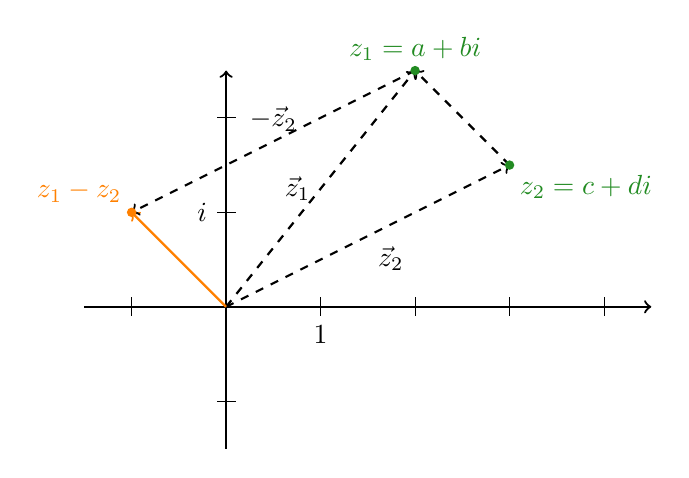
\begin{tikzpicture}[scale = 1.2]
  
        
        % Achsen mit Skala
        \draw[->, thick] (-1.5,0) -- (4.5,0) node[above] {$\RE$};
        \draw[->, thick] (0,-1.5) -- (0,2.5) node[right] {$\IM$};
        \foreach \x in {-1,2,3,4} 
            \draw (\x,0.1) -- (\x,-0.1) ;
        \foreach \y in {-1,2,} 
            \draw (0.1,\y) -- (-0.1,\y) ;
        \draw (0.1,1) -- (-0.1,1) node[left] {$i$};
        \draw (1,0.1) -- (1,-0.1) node[below] {$1$};
        
         % Vektoren
         \draw[->, thick, dashed] (0,0) -- node[left] {$\vec{z}_1$}  ++(2, 2.5) node[above, ForestGreen] {$z_1 = a + bi$};
         \draw[->, thick, dashed] (0,0) -- node[below right] {$\vec{z}_2$}  ++ (3,1.5) node[below right, ForestGreen] {$z_2 = c + di$};
         \draw[->, thick, orange] (0,0) -- (-1,1) node[above left, orange] {$z_1 - z_2$};
         \draw[->, thick, dashed] (2,2.5) -- node[above] {$-\vec{z}_2$}  ++(-3,-1.5) ; 
         \draw[->, thick, dashed] (3,1.5) -- (2,2.5) ; 
         
         % Punkte
         \fill[ForestGreen] (2,2.5) circle (0.05);
         \fill[ForestGreen] (3,1.5) circle (0.05);
         \fill[orange] (-1,1) circle (0.05);
    \end{tikzpicture}
    
\end{center}

\begin{center}
        
  
    Betrag
    
    \begin{tikzpicture}[scale = 1.2]
  
        
        % Achsen mit Skala
        \draw[->, thick] (-1.5,0) -- (4.5,0) node[above] {$\RE$};
        \draw[->, thick] (0,-1.5) -- (0,2.5) node[right] {$\IM$};
        \foreach \x in {-1,2,3,4} 
            \draw (\x,0.1) -- (\x,-0.1) ;
        \foreach \y in {-1,2,} 
            \draw (0.1,\y) -- (-0.1,\y) ;
        \draw (0.1,1) -- (-0.1,1) node[left] {$i$};
        \draw (1,0.1) -- (1,-0.1) node[below] {$1$};
        
         % Vektoren
         \draw[->, thick] (0,0) -- node[above] {$|z|$}  ++(2.5, 2) ;
         \draw[thick, orange] (0,0) -- node[below, orange] {$a$} ++(2.5,0) ;
         \draw[thick, orange] (2.5,0) -- node[right, orange] {$b$} ++(0,2);
              
         % Punkte
         \fill[ForestGreen] (2.5,2) circle (0.05) node[above, ForestGreen] {$z = a + bi$};
         
    \end{tikzpicture}
    
\end{center}

    


    
\end{multicols}

\clearpage
\begin{ueb}
    {}{}
    Gegeben sind zwei komplexe Zahlen $z$ und $w$. Bestimmen Sie die Summe $z+w$ und die Differenzen $z-w$, $w-2\bar{z}$ und $w-\frac{1}{2}z$ geometrisch durch Verknüpfen von Vektoren.

    \begin{center}
        
        \begin{tikzpicture}[scale = 1]
            % Gitter
            %\draw[dashed, very thin, gray] (-5,-5) grid (5,5);
            
            % Achsen mit Skala
            \draw[->, thick] (-5,0) -- (5,0) node[above] {$\RE$};
            \draw[->, thick] (0,-5) -- (0,5) node[right] {$\IM$};
            %\foreach \x in {-4,-3,-2,-1,1,2,3,4} 
            %    \draw (\x,0) -- (\x,-0.2) ;
            % \foreach \y in {-4,-3,-2, -1,2,3,4}
            %    \draw (0,\y) -- (-0.2,\y) ;
            %\draw (0,1) -- (-0.2,1) node[left] {$i$};
            %\draw (1,0) -- (1,-0.2) node[below] {$1$};
            
            % Punkte und Markierungen
            \fill[ForestGreen] (3,2) circle (0.1) node[left] {$z$};
            \fill[ForestGreen] (1,-2) circle (0.1) node[left] {$w$};

            %\fill[red] (4,0) circle (0.1) node[above] {z+w}
        \end{tikzpicture}
    \end{center}

\end{ueb}


\clearpage
\emph{Lösung}
\begin{center}
        
    \begin{tikzpicture}[scale = 1]
        % Gitter
        %\draw[dashed, very thin, gray] (-5,-5) grid (5,5);
        
        % Achsen mit Skala
        \draw[->, thick] (-5,0) -- (5,0) node[above] {$\RE$};
        \draw[->, thick] (0,-5) -- (0,5) node[right] {$\IM$};
        %\foreach \x in {-4,-3,-2,-1,1,2,3,4} 
        %    \draw (\x,0) -- (\x,-0.2) ;
        % \foreach \y in {-4,-3,-2, -1,2,3,4}
        %    \draw (0,\y) -- (-0.2,\y) ;
        %\draw (0,1) -- (-0.2,1) node[left] {$i$};
        %\draw (1,0) -- (1,-0.2) node[below] {$1$};
        
        % Punkte und Markierungen
        \fill[ForestGreen] (3,2) circle (0.1) node[left] {$z$};
        \fill[ForestGreen] (1,-2) circle (0.1) node[left] {$w$};

        \fill[red] (4,0) circle (0.1) node[above] {$z+w$};
        \fill[red] (2,4) circle (0.1) node[above] {$z-w$};
        \fill[red] (-0.5,-3) circle (0.1) node[above] {$w-\frac{1}{2}z$};
        \fill[red] (-5,2) circle (0.1) node[above] {$w-2\bar z$};
    \end{tikzpicture}
\end{center}





















\clearpage
\subsection{Die Polarform}

Ein Punkt in einem 2-dimensionalen Koordinatensystem ist durch die Angabe seiner kartesischen Koordinaten $x$ und $y$ eindeutig bestimmt. Ein Punkt kann auch durch den Winkel $\varphi$ (von der positiven $x$-Achse aus im Gegenuhrzeigersinn gemessen) und den Abstand $r$ (vom Ursprung) eindeutig bestimmt werden. Diese Darstellung heisst Polardarstellung.

\begin{center}
    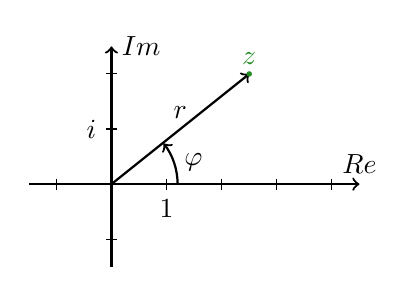
\begin{tikzpicture}[scale = 0.7]
        % Achsen mit Skala
        \draw[->, thick] (-1.5,0) -- (4.5,0) node[above] {$\operatorname{Re}$};
        \draw[->, thick] (0,-1.5) -- (0,2.5) node[right] {$\operatorname{Im}$};
        \foreach \x in {-1,2,3,4} 
            \draw (\x,0.1) -- (\x,-0.1) ;
        \foreach \y in {-1,2,} 
            \draw (0.1,\y) -- (-0.1,\y) ;
        \draw (0.1,1) -- (-0.1,1) node[left] {$i$};
        \draw (1,0.1) -- (1,-0.1) node[below] {$1$};
        
        % Vektoren
        \draw[->, thick] (0,0) -- node[above] {$r$}  ++(2.5, 2) ;
        
        % Punkte
        \fill[ForestGreen] (2.5,2) circle (0.05) node[above, ForestGreen] {$z$};
        
        % Winkel
        \draw[thick, ->] (1.2,0) arc (0:38:1.2) node[midway, right] {$\varphi$};
        
    \end{tikzpicture}   
\end{center}



\begin{definition}
    {Polarform}{}
    Jede komplexe Zahl $z \neq 0$ kann in der Polarform dargestellt werden als:

\begin{equation*}
    z = r \operatorname{cis} \varphi
\end{equation*}

Dabei bezeichnet $r$ den Abstand von $z$ zu $0$ und $\varphi$ den Winkel, der den zu $z$ gehörenden Ortsvektor mit der positiven $x$-Achse einschliesst. Man nennt $r$ den \textbf{Betrag} und $\varphi$ das \textbf{Argument} von $z$. Die Schreibweise dafür ist:

\begin{equation*}
    r = |z| \quad \text{und} \quad \varphi = \arg(z)
\end{equation*}

\end{definition}

\begin{bsp}
    {Polarform spezieller Zahlen}{}
    Polarformen von $1,i,-3,-4i, 1+i$

        
        \begin{tikzpicture}[scale = 0.7]
            % Gitter
            \draw[dashed, very thin, gray] (-5,-5) grid (5,5);
            
            % Achsen mit Skala
            \draw[->] (-5,0) -- (5,0) node[above] {$\RE$};
            \draw[->] (0,-5) -- (0,5) node[right] {$\IM$};
            \foreach \x in {-4,-3,-2,-1,1,2,3,4} 
                \draw (\x,0) -- (\x,-0.2) ;
            \foreach \y in {-4,-3,-2, -1,2,3,4} 
                \draw (0,\y) -- (-0.2,\y) ;
            \draw (0,1) -- (-0.2,1) node[left] {$i$};
            \draw (1,0) -- (1,-0.2) node[below] {$1$};
            
            % Punkte und Markierungen
            
        \end{tikzpicture}
 \vfill
\end{bsp}
\clearpage
Wie kann man die Polarform in die Normalform umrechnen? Betrachten Sie dazu das folgende Beispiel:
\begin{bsp}
    {Umrechnung Polarform $\rightarrow$ Normalform}{}

    Gegeben ist die Zahl $z = 4 \cis \left(\frac{\pi}{6}\right)$. 

    Gesucht ist die Normalform $z = a + bi$
  
        
        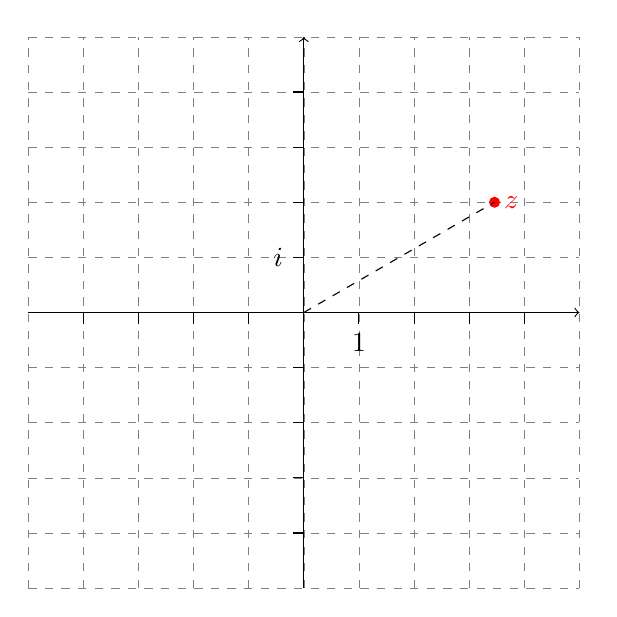
\begin{tikzpicture}[scale = 0.7]
            % Gitter
            \draw[dashed, very thin, gray] (-5,-5) grid (5,5);
            
            % Achsen mit Skala
            \draw[->] (-5,0) -- (5,0) node[above] {$\RE$};
            \draw[->] (0,-5) -- (0,5) node[right] {$\IM$};
            \foreach \x in {-4,-3,-2,-1,1,2,3,4} 
                \draw (\x,0) -- (\x,-0.2) ;
             \foreach \y in {-4,-3,-2, -1,2,3,4}
                \draw (0,\y) -- (-0.2,\y) ;
            \draw (0,1) -- (-0.2,1) node[left] {$i$};
            \draw (1,0) -- (1,-0.2) node[below] {$1$};
            
            % Punkte und Markierungen
             \fill[red] (2*1.73, 2) circle (0.1) node[right] {$z$};
             \draw[dashed] (0,0) -- ( 2*1.73, 2);
            
        \end{tikzpicture}
    
\end{bsp}
Wie kann man umgekehrt aus der Normalform die Polarform bestimmen?
\begin{bsp}
    {Umrechnung Normalform $\rightarrow$ Polarform}{}

    Gegeben ist die Zahl $z = 3 + 4i$. 

    Gesucht ist die Polarform $z = r \  \cis \varphi$
  
        
        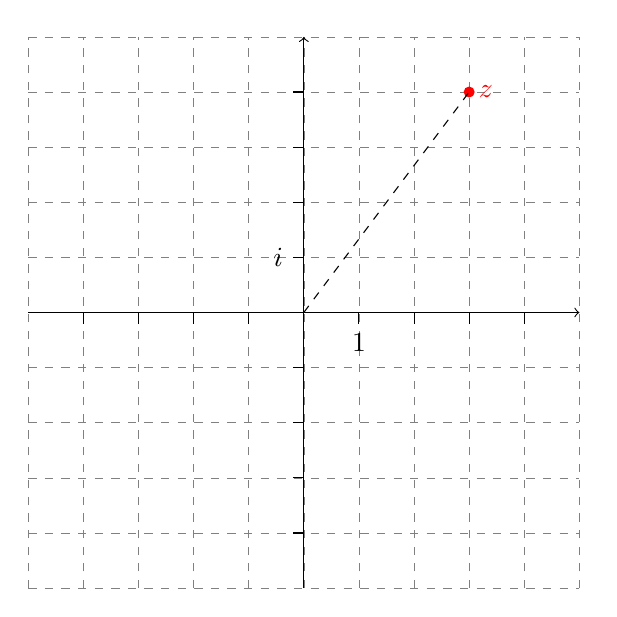
\begin{tikzpicture}[scale = 0.7]
            % Gitter
            \draw[dashed, very thin, gray] (-5,-5) grid (5,5);
            
            % Achsen mit Skala
            \draw[->] (-5,0) -- (5,0) node[above] {$\RE$};
            \draw[->] (0,-5) -- (0,5) node[right] {$\IM$};
            \foreach \x in {-4,-3,-2,-1,1,2,3,4} 
                \draw (\x,0) -- (\x,-0.2) ;
             \foreach \y in {-4,-3,-2, -1,2,3,4}
                \draw (0,\y) -- (-0.2,\y) ;
            \draw (0,1) -- (-0.2,1) node[left] {$i$};
            \draw (1,0) -- (1,-0.2) node[below] {$1$};
            
            % Punkte und Markierungen
            \fill[red] (3, 4) circle (0.1) node[right] {$z$};
            \draw[dashed] (0,0) -- ( 3, 4);
        \end{tikzpicture}
    
\end{bsp}
\clearpage
Vorsicht, wenn die gesuchte Zahl in der rechten Halbebene liegt:
\begin{bsp}
    {Umrechnung Normalform $\rightarrow$ Polarform }{}

    Gegeben ist die Zahl $z = -3 + 2i$. 

    Gesucht ist die Polarform $z = r \  \cis \varphi$
  
        
        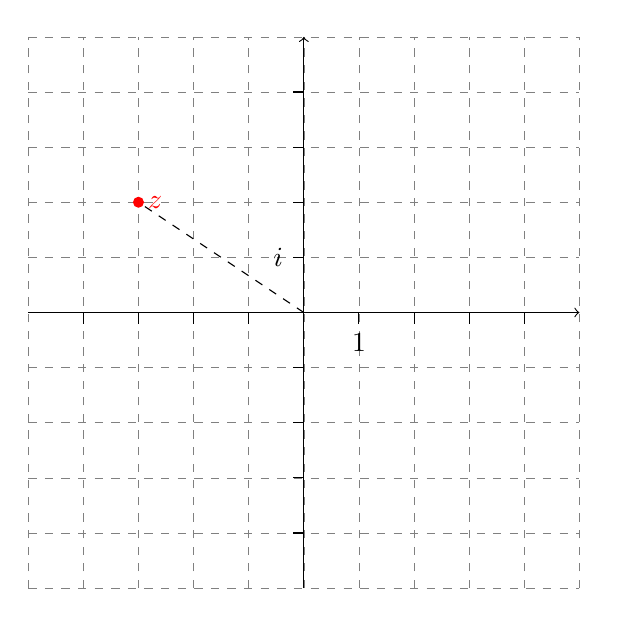
\begin{tikzpicture}[scale = 0.7]
            % Gitter
            \draw[dashed, very thin, gray] (-5,-5) grid (5,5);
            
            % Achsen mit Skala
            \draw[->] (-5,0) -- (5,0) node[above] {$\RE$};
            \draw[->] (0,-5) -- (0,5) node[right] {$\IM$};
            \foreach \x in {-4,-3,-2,-1,1,2,3,4} 
                \draw (\x,0) -- (\x,-0.2) ;
             \foreach \y in {-4,-3,-2, -1,2,3,4}
                \draw (0,\y) -- (-0.2,\y) ;
            \draw (0,1) -- (-0.2,1) node[left] {$i$};
            \draw (1,0) -- (1,-0.2) node[below] {$1$};
            
            % Punkte und Markierungen
            \fill[red] (-3, 2) circle (0.1) node[right] {$z$};
            \draw[dashed] (0,0) -- ( -3, 2);
        \end{tikzpicture}
    
\end{bsp}

\begin{satz}
    {Polarform $\rightarrow$ Normalform}{}
    Gegeben ist $z = r\ \cis(\varphi)$. Für die Normalform $z=a+bi$ gilt dann:
    $$ a = r \cos(\varphi), \qquad b = r\sin(\varphi)$$
    In anderen Worten:
    $$z  = r\cos(\varphi) + i \cdot r\sin(\varphi) =r \cdot \left( \cos(\varphi) + i \cdot \sin(\varphi)\right)$$

   (Die Bezeichnung $\cis$ ist eine Abkürzung für $\cos +\  i  \cdot \sin$)
\end{satz}

\begin{satz}
    {Normalform $\rightarrow$ Polarform}{}
    Gegeben ist $z = a + bi$. Für die Polarform $z = r\ \cis(\varphi)$ gilt dann
    $$r = |z| = \sqrt{a^2+b^2}$$

    $$\varphi = \arg (z) = \left\{ \begin{array}{ll}
            \frac{\pi}{2} & \text{, falls } a=0 \text{ und } b > 0 \\
            -\frac{\pi}{2} & \text{, falls } a=0 \text{ und } b < 0 \\
            \arctan\left(\frac{b}{a}\right) & \text{, falls $a>0$} \\
            \arctan\left(\frac{b}{a}\right) + \pi & \text{, falls $a<0$ } \\
    \end{array}\right.$$
    
\end{satz}

Es empfiehlt sich nicht, die Formel für die Berechnung des Arguments auswendig zu lernen. Stattdessen sollte man den betrachteten Punkt in der Zahlenebene skizzieren und sich in einer Skizze überlegen, welches der passende Winkel ist.



\begin{ueb}
    {}{}
    \begin{enumerate}
        \item Stellen Sie diese Zahlen in Normalform dar:
        \begin{multicols}{2}
            \begin{enumerate}
                \item[(a)] $2 \operatorname{cis}(0)$
                \item[(b)] $\operatorname{cis}\left(\frac{\pi}{3}\right)$
                \item[(c)] $\sqrt{2} \operatorname{cis}\left(\frac{3\pi}{2}\right)$
                \item[(d)] $5 \operatorname{cis}\left(-\frac{\pi}{6}\right)$
            \end{enumerate}
            \end{multicols}
        
        \item Stellen Sie die folgenden Zahlen in Polarform dar. Können Sie es auch ohne Taschenrechner? Ausser bei (p) sind es alles spezielle Winkel\dots 
        \begin{multicols}{2}
        \begin{enumerate}
            \item $2$
            \item $1 + i$
            \item $2 - 2i$
            \item $-1 + i$
            \item $-4 - 4i$
            \item $-\frac{1}{2} + \frac{\sqrt{3}}{2}i$
            \item $\frac{\sqrt{3}}{2} - \frac{1}{2}i$
            \item $-4$
            \item    $45$
            \item $-98$
            \item $77i$
            \item $-i$
            \item $-3 - 3i$
            \item $2 + 2\sqrt{3} i$
            \item $-3 + \sqrt{27} i$
            \item $-5 + 3i$
        \end{enumerate}
        \end{multicols}
        \item Stellen Sie die in beschreibender Form gegebene Zahlenmenge graphisch dar
        
            \begin{enumerate}
                \item[(a)] $\{ z \in \mathbb{C} \mid |z| = 1 \}$
                \item[(b)] $\{ z \in \mathbb{C} \mid |z| \geq \sqrt{5} \}$
                \item[(c)] $\{ z \in \mathbb{C} \mid \arg(z) = 45^\circ \}$
                \item[(d)] $\{ z \in \mathbb{C} \mid |z| < 3 \text{ und } \pi \leq \arg(z) \leq \frac{3\pi}{2} \}$
            \end{enumerate}
         
        \item Geben Sie von der zugehörigen Zahlenmenge eine beschreibende Form an.
        \begin{enumerate}
            \item[(a)] Kreislinie mit Zentrum $M = 0$ und Radius $R = 5$.
            \item[(b)] Kreisbogen mit dem Zentrum $M = 0$ und den Endpunkten $A = \sqrt{3} + i$ und $B = 1 + \sqrt{3} i$.
            \item[(c)] Gerade, die durch die Punkte $A = -1 - i$ und $B = 1 + i$ geht.
            \item[(d)] Strecke mit den Endpunkten $A = -\sqrt{3} + 3i$ und $B = -3\sqrt{3} + 9i$.
        \end{enumerate}
    \end{enumerate}
\end{ueb}


\begin{ueb}
    {Programmieraufgabe}{}
    Ergänzen Sie den Konstruktor \lstinline{__init__()} der Klasse `komplex' um das Attribut \lstinline{self.arg}, worin das Argument der komplexen Zahl gespeichert wird, sodass man mit \lstinline{z.arg} das Argument der Zahl $z$ erhält.



    Für die Verwendung von $\pi$ und $\arctan$ müssen diese zuerst importiert werden: \lstinline{from math import pi, atan}

    Ergänzen Sie anschliessend die Methode \lstinline{__str__()}, sodass bei Aufrufen von \lstinline{print(z)} sowohl die Normalform wie auch die Polarform in der Konsole ausgegeben wird.
\end{ueb}




\clearpage
\emph{Lösungen}
\begin{enumerate}
    \item Stellen Sie diese Zahlen in Normalform dar:
    \begin{enumerate}
        \item[(a)] $2$
        \item[(b)] $\frac{1}{2} + \frac{\sqrt{3}}{2}i$
        \item[(c)] $-\sqrt{2}i$
        \item[(d)] $\frac{5\sqrt{3}}{2} - \frac{5}{2}i$
    \end{enumerate}
    
    \item Stellen Sie die folgenden Zahlen in Polarform dar:
    \begin{enumerate}
        \item $2 \operatorname{cis}(0)$
        \item $\sqrt{2} \operatorname{cis}(\frac{\pi}{4})$
        \item $2\sqrt{2} \operatorname{cis}(-\frac{\pi}{4})$
        \item $\sqrt{2} \operatorname{cis}(\frac{3\pi}{4})$
        \item $4\sqrt{2} \operatorname{cis}(-\frac{3\pi}{4})$
        \item $ \operatorname{cis}(\frac{2\pi}{3})$
        \item $ \operatorname{cis}(-\frac{\pi}{6})$
        \item $4 \operatorname{cis}(\pi)$
        \item $45 \operatorname{cis}(0)$
        \item $98 \operatorname{cis}(\pi)$
        \item $77 \operatorname{cis}(\frac{\pi}{2})$
        \item $\operatorname{cis}(-\frac{\pi}{2})$
        \item $3\sqrt{2} \operatorname{cis}(-\frac{3\pi}{4})$
        \item $4 \operatorname{cis}(\frac{\pi}{3})$
        \item $6 \operatorname{cis}(\frac{2\pi}{3})$
        \item $\approx 5.83 \operatorname{cis}(2.11)$
    \end{enumerate}
    
    \item  \begin{multicols}{2}
        \begin{enumerate}
            \item $|z| = 1$
            \begin{center}
        
                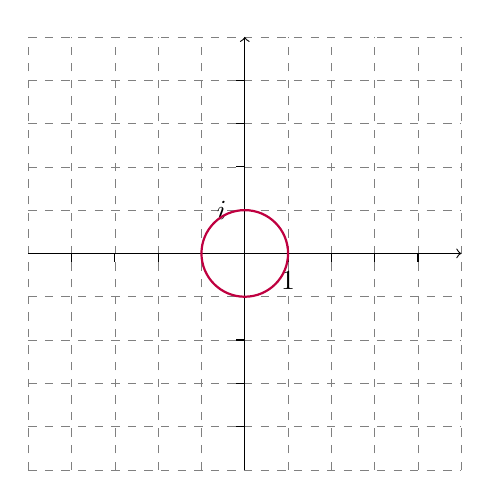
\begin{tikzpicture}[scale = 0.55]
                    % Gitter
                    \draw[dashed, very thin, gray] (-5,-5) grid (5,5);
                    
                    % Achsen mit Skala
                    \draw[->] (-5,0) -- (5,0) node[above] {$\RE$};
                    \draw[->] (0,-5) -- (0,5) node[right] {$\IM$};
                    \foreach \x in {-4,-3,-2,-1,1,2,3,4} 
                        \draw (\x,0) -- (\x,-0.2) ;
                     \foreach \y in {-4,-3,-2, -1,2,3,4}
                        \draw (0,\y) -- (-0.2,\y) ;
                    \draw (0,1) -- (-0.2,1) node[left] {$i$};
                    \draw (1,0) -- (1,-0.2) node[below] {$1$};
                    
                    % Punkte und Markierungen
                    \draw[thick, purple] (0,0) circle (1);
                \end{tikzpicture}
            \end{center}
            
            \item $|z| \ge 5$
            \begin{center}
        
                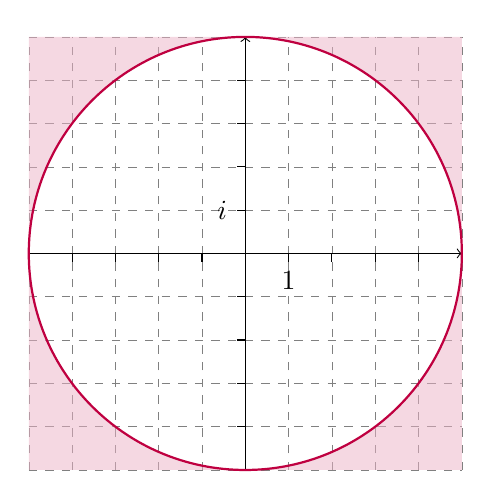
\begin{tikzpicture}[scale = 0.55]
                    % Gitter
                    \draw[dashed, very thin, gray] (-5,-5) grid (5,5);
                    
                    % Achsen mit Skala
                    \draw[->] (-5,0) -- (5,0) node[above] {$\RE$};
                    \draw[->] (0,-5) -- (0,5) node[right] {$\IM$};
                    \foreach \x in {-4,-3,-2,-1,1,2,3,4} 
                        \draw (\x,0) -- (\x,-0.2) ;
                     \foreach \y in {-4,-3,-2, -1,2,3,4}
                        \draw (0,\y) -- (-0.2,\y) ;
                    \draw (0,1) -- (-0.2,1) node[left] {$i$};
                    \draw (1,0) -- (1,-0.2) node[below] {$1$};
                    
                    % Punkte und Markierungen
                    \fill[even odd rule, purple!30, opacity=0.5] (-5,-5) rectangle (5,5) (0,0) circle (5);
                    \draw[thick, purple] (0,0) circle (5);              
                \end{tikzpicture}
            
            \end{center}

            \item $\arg(z) = 45^\circ$
            \begin{center}
        
                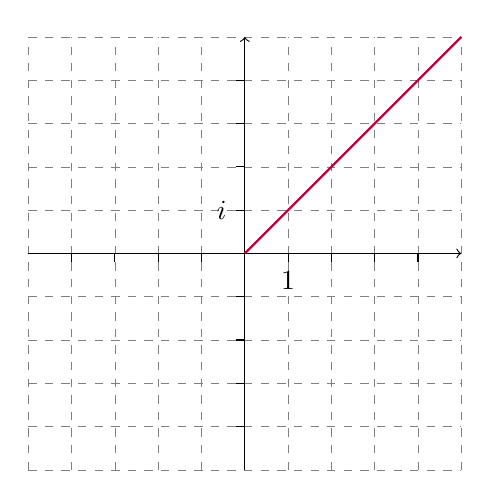
\begin{tikzpicture}[scale = 0.55]
                    % Gitter
                    \draw[dashed, very thin, gray] (-5,-5) grid (5,5);
                    
                    % Achsen mit Skala
                    \draw[->] (-5,0) -- (5,0) node[above] {$\RE$};
                    \draw[->] (0,-5) -- (0,5) node[right] {$\IM$};
                    \foreach \x in {-4,-3,-2,-1,1,2,3,4} 
                        \draw (\x,0) -- (\x,-0.2) ;
                     \foreach \y in {-4,-3,-2, -1,2,3,4}
                        \draw (0,\y) -- (-0.2,\y) ;
                    \draw (0,1) -- (-0.2,1) node[left] {$i$};
                    \draw (1,0) -- (1,-0.2) node[below] {$1$};
                    
                    % Punkte und Markierungen
                    \draw[thick, purple] (0,0) -- (5,5);
                \end{tikzpicture}
            \end{center}

            
            \item $|z|< 3$ und $\pi \le \arg(z)\le \frac{3\pi}{2}$
            \begin{center}
        
                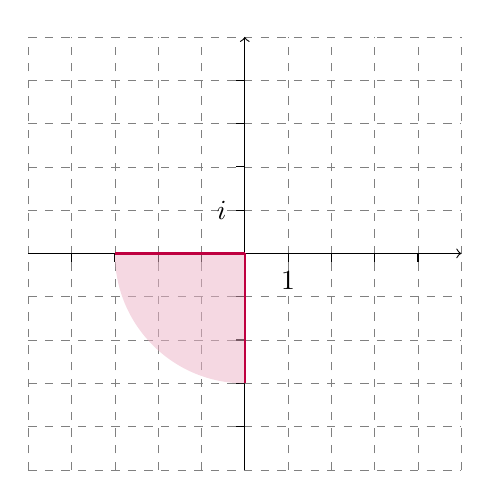
\begin{tikzpicture}[scale = 0.55, even odd rule]
                    % Gitter
                    \draw[dashed, very thin, gray] (-5,-5) grid (5,5);
                    
                    % Achsen mit Skala
                    \draw[->] (-5,0) -- (5,0) node[above] {$\RE$};
                    \draw[->] (0,-5) -- (0,5) node[right] {$\IM$};
                    \foreach \x in {-4,-3,-2,-1,1,2,3,4} 
                        \draw (\x,0) -- (\x,-0.2) ;
                     \foreach \y in {-4,-3,-2, -1,2,3,4}
                        \draw (0,\y) -- (-0.2,\y) ;
                    \draw (0,1) -- (-0.2,1) node[left] {$i$};
                    \draw (1,0) -- (1,-0.2) node[below] {$1$};
                    
                    % % Punkte und Markierungen
                    \fill[purple!30, opacity=0.5] (0,0) -- (-3,0) arc (180:270:3) -- cycle;
                    \draw[thick, purple] (0,0) -- (-3,0);
                    \draw[thick, purple] (0,0) -- (0,-3);
                    

                    % \fill[even odd rule, purple!30, opacity=0.5] (-5,-5) rectangle (5,5) (0,-1) circle (2);
                    % \draw[thick, purple] (0,-1) circle (2);

                \end{tikzpicture}
            \end{center}
            
        \end{enumerate}
        \end{multicols}

    
    \item Geben Sie von der zugehörigen Zahlenmenge eine beschreibende Form an:
    \begin{enumerate}
        \item[(a)] $\{z \in \mathbb{C} \mid |z| = 5 \}$
        \item[(b)] $\{z \in \mathbb{C} \mid |z| = 2 \text{ und } \frac{\pi}{6} \le \arg(z) \le \frac{\pi}{3}  \}$
        \item[(c)] $\{z \in \mathbb{C} \mid \arg(z) = \frac{\pi}{4} \text{ oder } \arg(z) = -\frac{3\pi}{4}\} \cup \{0\}$
        \item[(d)] $\{z \in \mathbb{C} \mid  2\sqrt{3}\le |z| \le 6\sqrt{3} \text{ und } \arg(z) = \frac{2\pi}{3} \}$
    \end{enumerate}
\end{enumerate}





























\clearpage
\subsection{Multiplikation und Division in Polarform}
\begin{LA}{}{}
    Gegeben sind die komplexen Zahlen:
\[
z_1 = \frac{3}{2} + \frac{3\sqrt{3}}{2} i, \quad z_2 = \sqrt{3} + i
\]

\begin{enumerate}
    \item Berechnen Sie \( z_3 = z_1 \cdot z_2 \).
    \item Berechnen Sie die Polarformen von \( z_1 \), \( z_2 \) und \( z_3 \).
    \item Welchen Zusammenhang besteht zwischen den Polarformen? Prüfen Sie Ihre Vermutung an weiteren, selbstgewählten Zahlenbeispiele.
\end{enumerate}
\vfill
\end{LA}

\pagebreak
\begin{satz}
    {Multiplikation in Polarform}{}
    Seien \( z_1 = r_1 \operatorname{cis} \varphi_1 \) und \( z_2 = r_2 \operatorname{cis} \varphi_2 \) zwei komplexe Zahlen. Dann gilt:

\[
z_1 \cdot z_2 = \hspace*{5 cm}
\]

\vspace{0.5cm}
\end{satz}

Für den Beweis dieser Rechenregel für Zahlen in Polarform, benötigen wir die Additionstheoreme für Sinus und Cosinus. Für beliebige Winkel $\alpha$ und $\beta$ gilt
$$ \sin(\alpha+\beta) = \sin(\alpha)\cos(\beta) + \cos(\alpha) \sin(\beta) \qquad \cos(\alpha+\beta) = \cos(\alpha)\cos(\beta) - \sin(\alpha)\sin(\beta) $$

\emph{Beweis:}
    
\vspace*{5cm}


Der Satz besagt, dass die Multiplikation mit einer komplexen Zahl $z_1 = r_1 \cis (\varphi_1)$ in der Zahlenebene wie eine Drehstreckung um das Zentrum $0$ wirkt: Wie die Abbildung illustriert, tritt dabei der Betrag $|z_1| = r_1$ als Streckfaktor auf und das Argument $\arg(z_1) = \varphi_1$ als Drehwinkel.


\begin{center}
    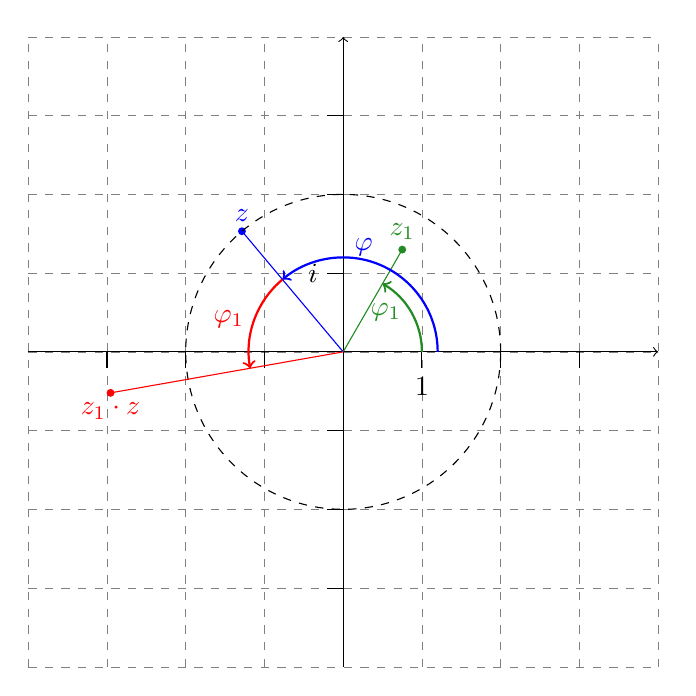
\begin{tikzpicture}[scale = 1]
        % Gitter
        \draw[dashed, very thin, gray] (-4,-4) grid (4,4);
                    
        % Achsen mit Skala
        \draw[->] (-4,0) -- (4,0) node[above] {$\RE$};
        \draw[->] (0,-4) -- (0,4) node[right] {$\IM$};
        \foreach \x in {-3,-2,-1,1,2,3} 
            \draw (\x,0) -- (\x,-0.2) ;
         \foreach \y in {-3,-2, -1,2,3}
            \draw (0,\y) -- (-0.2,\y) ;
        \draw (0,1) -- (-0.2,1) node[left] {$i$};
        \draw (1,0) -- (1,-0.2) node[below] {$1$};

        
        % Punkt z1
        \coordinate (z1) at (60:1.5);
        \fill[ForestGreen] (z1) circle (0.05) node[above, ForestGreen] {$z_1$};
        \draw[ForestGreen](0,0) -- (z1);
        \draw[thick, ->, ForestGreen] (1, 0) arc (0:60:1) node[midway, left] {$\varphi_1$};
        
         % Punkt z
         \coordinate (z) at (130:2);
         \fill[blue] (z) circle (0.05) node[above, blue] {$z$};
         \draw[blue](0,0) -- (z);
         \draw[thick, ->, blue] (1.2, 0) arc (0:130:1.2) node[midway, above left] {$\varphi$};
         \draw[dashed] (0,0) circle (2);

         % Punkt z_1*z
         \coordinate (z1z) at (190:3);
         \fill[red] (z1z) circle (0.05) node[below, red] {$z_1\cdot z$};
         \draw[red](0,0) -- (z1z);
         \draw[thick, ->, red] (130:1.2) arc (130:190:1.2) node[midway, left] {$\varphi_1$};
        
     
    \end{tikzpicture}   
\end{center}


\clearpage
Die wiederholte Multiplikation komplexer Zahlen auf dem Einheitskreis der Zahlenebene reduziert sich insbesondere zur wiederholten Addition ihrer Argumente. Dies hat den nach Abraham de Moivre (1667-1754) benannten Satz zur Folge:
\begin{satz}
{Satz von de Moivre 1}{}
Für jede komplexe Zahl $\cis(\varphi)$ auf dem Einheitskreis der Zahlenebene gilt:
$$(\cis(\varphi))^n = \cis(n\cdot\varphi)$$

\end{satz}



\begin{center}
    \begin{tikzpicture}[scale = 2]
        % Gitter
        \draw[dashed, very thin, gray] (-2,-2) grid (2,2);
                    
        % Achsen mit Skala
        \draw[->] (-2,0) -- (2,0) node[above] {$\RE$};
        \draw[->] (0,-2) -- (0,2) node[right] {$\IM$};
        \foreach \x in {-1,1} 
            \draw (\x,0) -- (\x,-0.2) ;
         \foreach \y in {-1}
            \draw (0,\y) -- (-0.2,\y) ;
        \draw (0,1) -- (-0.2,1) node[above left] {$i$};
        \draw (1,0) -- (1,-0.2) node[below right] {$1$};

        
     
        % Einheitskreis
        \draw[dashed] (0,0) circle (1);
         % Punkt z
         \coordinate (z) at (40:1);
         \fill[blue] (z) circle (0.05) node[above right, blue] {$z= \cis(\varphi)$};
         \draw[orange](0,0) -- (z);
         \draw[thick, ->, red] (0.5, 0) arc (0:40:0.5) node[midway, right] {$\varphi$};
         

         % Punkt z^2
         \coordinate (z2) at (80:1);
         \fill[blue] (z2) circle (0.05) node[above right, blue] {$z^2$};
         \draw[orange](0,0) -- (z2);
         \draw[thick, ->, red] (40:0.5) arc (40:80:0.5) node[midway, above right] {$\varphi$};
        
          % Punkt z^3
          \coordinate (z3) at (120:1);
          \fill[blue] (z3) circle (0.05) node[above left, blue] {$z^3$};
          \draw[orange](0,0) -- (z3);
          \draw[thick, ->, red] (80:0.5) arc (80:120:0.5) node[midway, above] {$\varphi$};
     
    \end{tikzpicture}   
\end{center}
Mit dem Satz von de Moivre lassen sich auch Potenzen von Zahlen berechnen, die nicht auf dem Einheitskreis liegen. Sei $z=r\cdot\cis(\varphi)$ eine beliebige Zahl. Dann gilt:
$$z^n=(r\cdot\cis(\varphi))^n = r^n \cdot(\cis(\varphi))^n = r^n\cdot\cis(n\cdot\varphi)$$

\begin{satz}
    {Satz von de Moivre 2}{}
    Für jede komplexe Zahl $z= r\cdot\cis(\varphi)$ gilt:
    $$z^n = r^n \cdot\cis(n\cdot\varphi)$$
    
    \end{satz}
\clearpage
\begin{ueb}
    {}{}
    \begin{enumerate}
        \item Berechne das Produkt und gib das Resultat in Normalform an.

        \begin{enumerate}
            \item \( \sqrt{2} \operatorname{cis}(43^\circ) \cdot \sqrt{18} \operatorname{cis}(77^\circ) \)
            \item \( 3 \operatorname{cis}(245^\circ) \cdot 13 \operatorname{cis}(25^\circ) \)
            \item \( 90 \operatorname{cis}(182^\circ) \cdot \frac{1}{5} \operatorname{cis}(223^\circ) \)
        \end{enumerate}
        
         \item Berechne $z^n$ für $z = \cos(60^\circ) + i \sin(60^\circ)$ und $n=2, n=3$ und $n=4245$.
        % \begin{enumerate}
        %     \item 
        %     % \item $z = 3 \operatorname{cis}(315^\circ)$
        % \end{enumerate}
    
        \item Berechne den Quotienten und gib das Resultat in Normalform an.
        \begin{enumerate}
            \item $\frac{87 \operatorname{cis}(105^\circ)}{29 \operatorname{cis}(15^\circ)}$
            \item $\frac{63 \operatorname{cis}(233^\circ)}{7 \operatorname{cis}(98^\circ)}$
            \item $\frac{\sqrt{2} \operatorname{cis}(5^\circ)}{2 \operatorname{cis}(215^\circ)}$
        \end{enumerate}
    
        \item Berechne den folgenden Quotienten. Entscheide, ob du in Normal- oder Polarform rechnen willst. Gib das Resultat in Normalform an.
        \begin{enumerate}
            \item $w = \frac{\operatorname{cis}(45^\circ)}{\operatorname{cis}(105^\circ)}$
            \item $w = \frac{4 + 4i}{2 \operatorname{cis}(135^\circ)}$
        \end{enumerate}
    
        % \item Gegeben ist die Zahl $z = 3 \operatorname{cis}(15^\circ)$. Berechne für die folgenden Zahlen $w$ jeweils $wz$ und $\frac{z}{w}$ und beschreibe die gegenseitige Lage von $z$ und $w$.
        % \begin{enumerate}
        %     \item $w = 2$
        %     \item $w = \frac{1}{2}$
        %     \item $w = \operatorname{cis}(45^\circ)$
        %     \item $w = 2i$
        % \end{enumerate}

        \item In der Skizze sind die Zahlen $z$ und $w\cdot z$ abgebildet. Wo muss de Zahl $w$ liegen?.
        

\begin{center}
    \begin{tikzpicture}[scale = 1]
        % Gitter
        %\draw[dashed, very thin, gray] (-4,-4) grid (4,4);
                    
        % Achsen mit Skala
        \draw[->] (-4,0) -- (4,0) node[above] {$\RE$};
        \draw[->] (0,-4) -- (0,4) node[right] {$\IM$};
        \foreach \x in {-3,-2,-1,1,2,3} 
            \draw (\x,0) -- (\x,-0.2) ;
         \foreach \y in {-3,-2, -1,2,3}
            \draw (0,\y) -- (-0.2,\y) ;
        \draw (0,1) -- (-0.2,1) node[left] {$i$};
        \draw (1,0) -- (1,-0.2) node[below] {$1$};

        
        % Punkt z
        \coordinate (z) at (310:1);
        \fill[ForestGreen] (z) circle (0.05) node[above, ForestGreen] {$z$};
        % \draw[ForestGreen](0,0) -- (z1);
        % \draw[thick, ->, ForestGreen] (1, 0) arc (0:60:1) node[midway, left] {$\varphi_1$};
        
         % Punkt wz
         \coordinate (wz) at (70:3);
         \fill[blue] (wz) circle (0.05) node[above, blue] {$wz$};
        %  \draw[blue](0,0) -- (z);
        %  \draw[thick, ->, blue] (1.2, 0) arc (0:130:1.2) node[midway, above left] {$\varphi$};
        %  \draw[dashed] (0,0) circle (2);

         % Punkt w
        %  \coordinate (w) at (120:3);
        %  \fill[red] (w) circle (0.05) node[below, red] {$w$};
        %  \draw[red](0,0) -- (z1z);
        %  \draw[thick, ->, red] (130:1.2) arc (130:190:1.2) node[midway, left] {$\varphi_1$};
        
     
    \end{tikzpicture}   
\end{center}

    
        % \item Gib zur Zahl $z$ die konjugiert komplexe Zahl $\bar{z}$ und die Gegenzahl $-z$ in Polarform an.
        % \begin{enumerate}
        %     \item $4 \operatorname{cis}(60^\circ)$
        %     \item $\frac{1}{3} \operatorname{cis}(45^\circ)$
        % \end{enumerate}

\clearpage

        \item Die Polarform ist beim Multiplizieren, Dividieren und Potenzieren von Vorteil. Die Normalform hingegen bei Addition und Subtraktion.  
        Gegeben seien die komplexen Zahlen:
        
        \[
        v = 2 \operatorname{cis} \left(\frac{5\pi}{6}\right), \quad w = 3 \operatorname{cis} \left(\frac{3\pi}{4}\right), \quad z = 4 \operatorname{cis} \left(\frac{\pi}{12}\right)
        \]
        
        Berechne und gib das Resultat in Normalform an:
        
        \begin{enumerate}
            \item \( \frac{v \cdot w}{z} \)
            %\item \( w^{-3} \)
            \item \( \frac{z^2}{v^5} \)
            \item \( v + w \cdot z \)
        \end{enumerate}
        
    
        \item Es sind $z_1 = 3 + 6i$, $z_2 = -1 + 2i$, $z_3 = -12i$. Berechne:
        \begin{enumerate}
            \item $\arg(z_1 - z_2)$
            \item $|z_1 + 2i \cdot z_2|$
            \item $\arg \left( \frac{z_1}{z_3} \right)$
            \item $\arg(z_1^2 \cdot z_2)$
            \item $\left|\frac{z_1}{12 + z_2}\right|$
            \item $\arg \left( \frac{z_2 + 3}{z_1} \right)$
        \end{enumerate}

        \item Berechne $(1+i)^6 + (1-i)^6$ und gib das Resultat in Normalform an.
    
        \item Berechne die folgenden Terme. Entscheide dabei, ob du in Polar- oder Normalform rechnen willst. Gib die Ergebnisse in Normal- und Polarform an.
        \begin{enumerate}
            \item $\left( \frac{2 - 2i}{1 + i} \right)^3$
            \item $\left( \frac{1 + \sqrt{3} i}{\sqrt{3} - i} \right)^4$
            \item $\frac{(1 - \sqrt{3} i)^9}{(-1 + i)^{15}}$
            \item $\left( \frac{2 - 2i}{1 + \sqrt{3} + (1 - \sqrt{3}) i} \right)^3$
        \end{enumerate}
    \end{enumerate}
\end{ueb}

\clearpage
\emph{Lösungen}

\begin{enumerate}
    \item Berechne das Produkt und gib das Resultat in Normalform an.
    \begin{enumerate}
        \item $-3+3\sqrt{3}i$
        \item $-39i$
        \item $9\sqrt{2}+9\sqrt{2}i$
    \end{enumerate}


    \item Berechne $z^n$ in der Polarform:
    $$ z^2 = \operatorname{cis}(120^\circ) = -\frac{1}{2} + \frac{\sqrt{3}}{2}i, \quad z^3 = \operatorname{cis}(180^\circ) = -1, \quad z^{4245} = z^3 = \cis(180^\circ) = -1$$
    % \begin{enumerate}
    %     \item $\operatorname{cis}(120^\circ), \operatorname{cis}(180^\circ), \operatorname{cis}(240^\circ), \operatorname{cis}(300^\circ), \operatorname{cis}(0^\circ) z^7 = z, \quad z^8 = z^2, \quad z^9 = z^3, \quad z^{10} = z^4$
    %     \item $9 \operatorname{cis}(270^\circ), 27 \operatorname{cis}(225^\circ), 81 \operatorname{cis}(180^\circ), 243 \operatorname{cis}(135^\circ),729 \operatorname{cis}(90^\circ), 2187 \operatorname{cis}(45^\circ), 6561 \operatorname{cis}(0^\circ), z^9 = 6561z, \quad z^{10} = 6561z^2$
    % \end{enumerate}

    \item Berechne den Quotienten:
    \begin{enumerate}
        \item $3 i$
        \item $-9\frac{\sqrt{2}}{2} +9\frac{\sqrt{2}}{2}i$
        \item $-\frac{\sqrt{6}}{4}+ \frac{\sqrt{2}}{4}i$
    \end{enumerate}

    \item Berechne $w$ in Normalform:
    \begin{enumerate}
        \item $w = \operatorname{cis}(-60^\circ) = \frac{1}{2} - \frac{\sqrt{3}}{2} i$
        \item $w = \frac{4 \sqrt{2} \operatorname{cis}(45^\circ)}{2 \operatorname{cis}(135^\circ)} = 2\sqrt{2} \operatorname{cis}(-90^\circ) = -2\sqrt{2}i$
    \end{enumerate}

    \item $w$ zeichnen
    \begin{center}
        \begin{tikzpicture}[scale = 1]
            % Gitter
            %\draw[dashed, very thin, gray] (-4,-4) grid (4,4);
                        
            % Achsen mit Skala
            \draw[->] (-4,0) -- (4,0) node[above] {$\RE$};
            \draw[->] (0,-4) -- (0,4) node[right] {$\IM$};
            \foreach \x in {-3,-2,-1,1,2,3} 
                \draw (\x,0) -- (\x,-0.2) ;
             \foreach \y in {-3,-2, -1,2,3}
                \draw (0,\y) -- (-0.2,\y) ;
            \draw (0,1) -- (-0.2,1) node[left] {$i$};
            \draw (1,0) -- (1,-0.2) node[below] {$1$};
    
            
            % Punkt z
            \coordinate (z) at (310:1);
            \fill[ForestGreen] (z) circle (0.05) node[above, ForestGreen] {$z$};
            % \draw[ForestGreen](0,0) -- (z1);
            % \draw[thick, ->, ForestGreen] (1, 0) arc (0:60:1) node[midway, left] {$\varphi_1$};
            
             % Punkt wz
             \coordinate (wz) at (70:3);
             \fill[blue] (wz) circle (0.05) node[above, blue] {$wz$};
            %  \draw[blue](0,0) -- (z);
            %  \draw[thick, ->, blue] (1.2, 0) arc (0:130:1.2) node[midway, above left] {$\varphi$};
            %  \draw[dashed] (0,0) circle (2);
    
             % Punkt w
             \coordinate (w) at (120:3);
             \fill[red] (w) circle (0.05) node[below, red] {$w$};
            %  \draw[red](0,0) -- (z1z);
            %  \draw[thick, ->, red] (130:1.2) arc (130:190:1.2) node[midway, left] {$\varphi_1$};
            
         
        \end{tikzpicture}   
    \end{center}

    % \item Berechne $wz$ und $\frac{z}{w}$ für verschiedene Werte von $w$:
    % \begin{enumerate}
    %     \item $wz = 6 \operatorname{cis}(15^\circ), \quad \frac{z}{w} = \frac{3}{2} \operatorname{cis}(15^\circ)$ Multiplikation mit 2 bedeutet Streckung mit dem Faktor 2, Division Stauchung auf die Hälfte. Der Winkel        ändert sich nicht.
    %     \item $wz = \frac{3}{2} \operatorname{cis}(15^\circ), \quad \frac{z}{w} = 6 \operatorname{cis}(15^\circ)$ Multiplikation mit 1/2 bedeutet Stauchung auf die Hälfte, Division Streckung mit dem Faktor 2. Der Winkel
    %     ändert sich nicht.
    %     \item $wz = 3 \operatorname{cis}(60^\circ), \quad \frac{z}{w} = 3 \operatorname{cis}(330^\circ)$ Multiplikation mit $\cis(45^\circ)$ bedeutet eine Drehung gegen den Uhrzeigersinn um 45 Grad, Division ist eine Drehung im Uhrzeigersinn.
    %     \item $wz = 6 \operatorname{cis}(105^\circ), \quad \frac{z}{w} = \frac{3}{2} \operatorname{cis}(285^\circ)$ Multiplikation mit $2i$ bedeutet Streckung mit dem Faktor 2 und Drehung um 90 Grad gegen den Uhrzeigersinn.
    %     Division bedeutet Stauchung und Drehung im Uhrzeigersinn.
    % \end{enumerate}

    % \item Konjugierte und Gegenzahl in Polarform:
    % \begin{enumerate}
    %     \item $\bar{z} = 4 \operatorname{cis}(300^\circ), \quad -z = 4 \operatorname{cis}(240^\circ)$
    %     \item $\bar{z} = \frac{1}{3} \operatorname{cis}(315^\circ), \quad -z = \frac{1}{3} \operatorname{cis}(225^\circ)$
    % \end{enumerate}

    \item  \begin{enumerate}
            \item $-\frac{3}{2}i$
            %\item $\frac{\sqrt{2}}{54} - \frac{\sqrt{2}}{54}i $
            \item $\frac{1}{2}$
            \item $-7\sqrt{3}+7i$
         \end{enumerate}
    \item Berechne die Winkel oder Werte:
    \begin{enumerate}
        \item $45^\circ$
        \item $\sqrt{17}$
        \item $\approx 153.43^\circ$
        \item $\approx 243.43^\circ$
        \item $\frac{3}{5}$
        \item $\approx 341.57^\circ$
    \end{enumerate}
    \item $0$
    \item Berechne
    \begin{enumerate}
        \item $8i = 8 \operatorname{cis}(90^\circ)$
        \item $1 = \operatorname{cis}(0^\circ)$
        \item $2 - 2i = 2\sqrt{2} \operatorname{cis}(-45^\circ)$
        \item $-i = \operatorname{cis}(270^\circ)$
    \end{enumerate}



\end{enumerate}

